\documentclass[lettersize,journal]{IEEEtran}

\usepackage{amsmath,amsfonts,amssymb}
\usepackage{algorithmic}
\usepackage{array}
\usepackage{textcomp}
\usepackage{stfloats}
\usepackage{url}
\usepackage{verbatim}
\usepackage{graphicx}
\usepackage{cite}
\usepackage{balance}
\newtheorem{theorem}{Theorem}
\newtheorem{proposition}{Proposition}
\newtheorem{lemma}{Lemma}
\newtheorem{corollary}{Corollary}
\newtheorem{remark}{Remark}
\newtheorem{assumption}{Assumption}
\hyphenation{op-tical net-works semi-conduc-tor IEEE-Xplore}
\def\BibTeX{{\rm B\kern-.05em{\sc i\kern-.025em b}\kern-.08em
    T\kern-.1667em\lower.7ex\hbox{E}\kern-.125emX}}

\urlstyle{same}
\begin{document}

\title{Multirobot Tracking of Separatrices and
Objective Eulerian Coherent Structures}

\author{Christopher Waight and Christopher A. Kitts,~\IEEEmembership{Senior Member,~IEEE}
\thanks{C. Waight is a PhD Candidate in the Robotic Systems Laboratory, Department of Mechanical Engineering, Santa Clara University, Santa Clara, CA 95053 USA (e-mail: cwaight@scu.edu)}
\thanks{C. A. Kitts is Professor and Director of the Robotic Systems Laboratory, Department of Mechanical Engineering, Santa Clara University, Santa Clara, CA 95053 USA (e-mail: ckitts@scu.edu)}
}
\markboth{IEEE Transactions on Robotics}%
{Waight and Kitts: Multirobot Tracking of Separatrices and Objective Eulerian Coherent Structures}

\maketitle

\begin{abstract}
Short-term transport in a geophysical flow is organized by
instantaneous coherent structures: curves of strongest local attraction
and repulsion, where drifting material collects within hours. Existing
robotic trackers either commit to a presumed structure in advance or
must integrate measurements over a time horizon before an estimate
exists. This paper presents a multirobot method for finding and
following these structures in real time, using only the instantaneous flow velocity
each robot measures at its own position. A cooperative estimator
recovers the local quadratic model of the field from one synchronous
measurement set, and six robots are proved to be the minimum team for
this recovery under the unconstrained quadratic model. The fit supplies two trackable surrogates. The first is the Jacobian
determinant, whose valley lines trace the flow's separatrices; it is
Galilean invariant but not objective, shifting under a rotating observer.
The second is the smaller rate-of-strain eigenvalue, whose trench is
objective, a material curve recovered identically in any observer frame.
An adaptive navigation controller rides each. A rotating-frame experiment
separates them: the strain tracker's inertial and rotating runs end
0.025 apart, while the determinant tracker's diverge by 1.219 as its
rotating-frame run leaves the structure. This objectivity has a
measurable cost in convergence rate and in noise tolerance at a single
decision point. Monte Carlo sweeps place the determinant
tracker's failure cliff at the estimator's own noise threshold,
$\sigma_{uv} \approx 0.01$, and the strain tracker's earlier, at
$\sigma_{uv} \approx 0.002$; at zero noise their tracking errors are
0.0016 and 0.0075. On Santa Barbara Channel radar currents, the
determinant tracker follows a coherent ridge for 28 hours to a consistent
landfall, and the strain tracker, started on that same ridge, rides the
same network structure from the objective strain term alone. Double-gyre
quantities are reported in the field's non-dimensional world units
throughout.
\end{abstract}

\begin{IEEEkeywords}
Multirobot Systems, Adaptive Navigation, Coherent Structures,
Okubo-Weiss, Rate of Strain, Objectivity, Cooperative
Estimation, Cluster Space Control
\end{IEEEkeywords}

\section{Introduction}
\label{sec:intro}

\IEEEPARstart{M}{ultirobot} systems provide redundancy against
individual failures, widen the area a team can cover, and spread
sensing across space rather than concentrating it at a single
platform. These systems now operate across domains from warehousing
to search and rescue \cite{1}. Equipped with field sensors, such
teams form mobile sensor networks that turn spatial spread into
simultaneous measurements at separated points.

Survey-oriented navigation use this ability to sweep a region exhaustively and identifying features only
afterward. Adaptive navigation (AN) techniques instead use
measurements in real time to drive the network toward or along
features of interest, locating local features quickly and following
them as they evolve.

AN in scalar fields is well developed. Each robot contributes a single
scalar measurement to a navigation policy that reaches and follows
features such as extrema, contour lines, ridges, trenches, saddle
points, and fronts \cite{26,27,28,29}, with formations sized so that
differential measurements across the cluster recover the gradient and
curvature each policy consumes \cite{15,26}.

Some environments are better modeled by vector fields. These models
assign both a magnitude and a direction to each point. The critical
points of that vector field often mark the features a mission cares
about, for example, in ocean currents and other geophysical flows. A
sink, for instance, can flag an area of high probability for search
and rescue, while a spewing vortex can point to a below-surface leak.
In \cite{14}, a three-robot cluster estimated the location and type of
an isolated critical point from a linear fit of simultaneous local
velocity measurements, recovering the feature from instantaneous data
alone rather than from an accumulated survey.

Beyond isolated points, there is also utility in tracking extended
features such as fronts, dynamically meaningful lines along which
water masses converge. Coordinated multi-vehicle sampling of such
dynamic ocean features is itself an active area of marine robotics,
spanning drifter-referenced AUV surveys \cite{2}, front-tracking
ASV/AUV teams \cite{3}, and adaptive glider fleets \cite{4}.

Another line of great interest is the separatrix. In steady
two-dimensional flows it is the union of the stable and unstable
manifolds through the saddle points, partitioning the domain into
basins whose trajectories do not mix. Tracking it is relevant to
dispersion modeling, pollutant containment, and coastal sensor
deployment \cite{6,7,8}, and, like the related Okubo-Weiss field used
to classify oceanic mesoscale eddies \cite{5}, it can in principle be
inferred from instantaneous measurements alone.

A line of work on separatrix navigation has equipped robot teams to
track a coherent structure directly in the flow rather than
reconstruct it offline, by straddling a presumed manifold with a small
formation \cite{9,10,11,12} or by accumulating an onboard FTLE
estimate over a finite time horizon \cite{13}. Each approach either
commits to the structure's identity before tracking begins or pays an
integration latency before an estimate exists.

This paper's approach requires neither pre-straddling an assumed
manifold nor accumulation of data points. From an arbitrary six-robot
configuration, the team infers a structure's location, its type, and,
at a crossing, which branch to continue onto, from the current
instantaneous measurement alone. The technique exploits the fact that
the velocity gradient splits uniquely into strain plus spin,
$\mathbf{J} = \mathbf{S} + \mathbf{W}$, and that for incompressible
planar flow the determinant splits with it, $D = \omega^2/4 - s_1^2$,
where $\omega$ is the vorticity carried by $\mathbf{W}$ and $s_1$ the
smaller eigenvalue of $\mathbf{S}$.
Each term is a trackable surrogate of the flow's transport skeleton,
and each controller developed here rides one of them. The former surrogate 
is Galilean invariant while the latter is objective.

This paper makes four contributions. First, it presents a cooperative
second-order estimator that recovers the local quadratic model of a
two-component field from one synchronous sample, with six robots proved
minimal for the unconstrained quadratic model and with exact,
heading-isotropic noise gains. Second, it
develops the $D$ tracker, a hybrid controller built on a modified
Newton step that snaps onto a trench of $D$, slides along it, and
traverses the network of saddle crossings without committing to a
manifold identity in advance. Third, it develops the
$s_1$ tracker, an objective controller built from the strain
eigenframe whose design follows from the structural result that no
quadratic velocity fit can certify $s_1$-trench curvature; on the
double gyre it captures reliably at a terminal core rather than
continuing past it, resolving both the attracting/repelling eigenvector
swap and the network crossing itself from objective quantities alone,
and on a field without a stationary point close enough to trigger that
capture it instead traverses the ridge network the strain term itself
resolves. Fourth, it validates both trackers under a fully specified
noise model, in a closed-loop rotating-frame objectivity experiment,
and on real Santa Barbara Channel radar currents.

The remainder of the paper is organized as follows. The rest of this
section reviews related work. Section~\ref{sec:detj_field} formulates
the problem. Section~\ref{sec:estimation} develops the six-robot
estimator and its accuracy under noise. Section~\ref{sec:controllers}
presents the two controllers and their stability properties, with
proofs in Appendix~\ref{app:proofs}. Section~\ref{sec:methods}
describes the simulation program and test plan, and
Section~\ref{sec:results} presents results, including the ocean
experiments. Section~\ref{sec:discussion} discusses implications and
limitations, and Section~\ref{sec:conclusion} concludes.

\subsection{Related Work}
\label{sec:related_robots}

Haller and Yuan formalized the Lagrangian coherent structure (LCS) as
the generalization of stable and unstable manifolds to flows with
arbitrary time dependence \cite{6}. The standard computable definition,
a ridge of the finite-time Lyapunov exponent (FTLE) field, is given in
\cite{8} on the same double-gyre model used throughout this paper. The
objectivity and Lagrangian/Eulerian tradeoff that bears on any Eulerian
surrogate is developed in \cite{16,17,18}. Velocity-gradient
recovery from sparse trajectories \cite{19} and the strain-spin
decomposition itself \cite{20} remain active adjacent directions. The
instantaneous criteria remain the computable workhorses: Okubo and Weiss
partition a planar flow from the local velocity gradient alone
\cite{21,22}, generalized to three dimensions \cite{23}, refined for
oceanographic use \cite{24}, and used at scale in mesoscale eddy censuses
\cite{5}.

The nearest prior work tracks a coherent structure directly with a
robot formation. Michini et al. bracket a presumed stable or unstable
manifold with three robots using only local velocity measurements
\cite{9}; the strategy extends to $N$ robots \cite{10}, was validated
on micro surface vehicles in a flow tank \cite{11}, and related
flow-based control operates marine robots in gyre-like environments
\cite{12}. Unlike methods that sense only a scalar reduction of the
field \cite{25}, the team here fits the full local quadratic vector
field, so the surrogate's shape, not merely its sign, is available to
the controllers. The straddle family commits to the manifold's identity
before tracking begins, and neither controller nor proof addresses the
saddle point itself, exactly where that identity becomes ambiguous.
Kularatne and Hsieh instead compute the local FTLE field on board,
recovering the structure's type at the price of a nonzero integration
horizon \cite{13}. None of these strategies estimates the curvature of
the field itself, which is what fixes not just where a structure lies
but what kind it is and how many branches meet there.

On the estimation side, \"{O}gren, Fiorelli, and Leonard established
cooperative gradient climbing with a formation of mobile sensors
\cite{26}, and Bri\~{n}\'{o}n-Arranz, Renzaglia, and Schenato extended
the idea to the Hessian: five robots on a ring plus one at the center
recover the gradient and Hessian of a scalar signal in closed form
\cite{15}. McDonald, Kitts, and Neumann developed the complementary
adaptive-navigation primitives that follow scalar-field ridges,
trenches, and saddle points from local differences alone
\cite{27,28,29}. Every one of these formations samples a single signal
channel. A coupled two-component field doubles the estimation problem
to twelve unknowns, which none of these formations addresses. Where
\cite{15} applies fixed symmetric weights valid
for the ideal ring geometry, the estimator here solves at the measured
positions and so stays exact even as the formation deforms. On the
control side, the step used here normalizes the Newton component by the
magnitude of the curvature in each eigendirection, a substitution that
also appears in the saddle-free method of Dauphin et al. \cite{35},
and takes the direction of the along-trench motion from the ambient
flow. The purpose differs: \cite{35} uses the substitution to escape
stationary points, while both trackers developed here are built to
find and hold them.

This paper and the critical-point and structure-tracking methods above
\cite{9,10,11,12,13,14} navigate a naturally occurring flow sensed in
situ, unlike the separate literature that builds an artificial vector
field as a synthetic guidance signal for single-robot path following
\cite{37} or obstacle avoidance \cite{38}.

\section{Problem Formulation}
\label{sec:detj_field}

\subsection{Vector Fields and Local Polynomial Models}

A planar vector field assigns a velocity vector $\mathbf{v}(\mathbf{p}) =
(u(\mathbf{p}), v(\mathbf{p}))$ to each position $\mathbf{p} = (x, y)$ in its
domain. The critical-point estimator of \cite{14} fits a \emph{planar}
(affine) model of each component to simultaneous measurements and solves
the linear system for the point where $\mathbf{v} = \mathbf{0}$. The
surrogates this paper tracks are built not from $\mathbf{v}$ but from its
spatial derivatives, and navigating them requires derivatives through
second order; a planar fit, whose second derivatives are identically zero,
cannot supply them.

The team therefore works from the second-order Taylor expansion of each
component about the cluster centroid $\mathbf{p}_c$. Coordinates
$\mathbf{p} = (x, y)$ are measured from the centroid throughout this
section, so that $\mathbf{p} = \mathbf{0}$ is the centroid itself:
\begin{align}
    u(\mathbf{p}) &= a_1 + a_2 x + a_3 y
        \nonumber \\
        &\quad + a_4 xy + \tfrac{1}{2} a_5 x^2 + \tfrac{1}{2} a_6 y^2
        + \mathcal{O}(\|\mathbf{p}\|^3),
        \label{eq:quad_model_u} \\
    v(\mathbf{p}) &= b_1 + b_2 x + b_3 y
        \nonumber \\
        &\quad + b_4 xy + \tfrac{1}{2} b_5 x^2 + \tfrac{1}{2} b_6 y^2
        + \mathcal{O}(\|\mathbf{p}\|^3).
        \label{eq:quad_model_v}
\end{align}
The twelve coefficients are constants; all position dependence in
(\ref{eq:quad_model_u})--(\ref{eq:quad_model_v}) is carried by $x$ and
$y$. Each coefficient is a derivative of the field at the centroid, and
the one-half factors are chosen so that the match is direct:
$a_1 = u(\mathbf{p}_c)$, $a_2 = \partial u/\partial x|_{\mathbf{p}_c}$,
$a_4 = \partial^2 u/\partial x \partial y|_{\mathbf{p}_c}$,
$a_5 = \partial^2 u/\partial x^2|_{\mathbf{p}_c}$, and likewise for
$b_1, \ldots, b_6$ with $v$ in place of $u$. Where a partial derivative
of the true field is meant rather than a fitted coefficient, this paper
writes it as a derivative: $u_x$, $u_{xy}$, and so on.

The team estimates these coefficients by fitting the quadratic model that
remains when the $\mathcal{O}(\|\mathbf{p}\|^3)$ remainder is discarded,
and marks the results with a hat: $\hat{a}_5$ is an estimate of $a_5$,
not the quantity itself. Two mechanisms separate them. Sensor
noise perturbs each measurement, and truncation bias arises because the
discarded cubic terms are not zero over a footprint of finite size, so the
fit absorbs part of them into the retained coefficients.

The first-order coefficients are the centroid values of the entries of the
field Jacobian
\begin{equation}
    \mathbf{J}(\mathbf{p}) =
    \begin{bmatrix}
        \partial u / \partial x & \partial u / \partial y \\
        \partial v / \partial x & \partial v / \partial y
    \end{bmatrix},
    \label{eq:jacobian}
\end{equation}
so that $\mathbf{J}_0 = \mathbf{J}(\mathbf{p}_c)$ has entries $a_2$,
$a_3$, $b_2$, $b_3$, and we write $D(\mathbf{p}) =
\det(\mathbf{J}(\mathbf{p}))$ throughout. 

\label{sec:separatrix}
\subsection{Surrogate I: the Okubo-Weiss Field $D$}

The Okubo-Weiss parameter \cite{21,22}, built from the normal strain,
shear strain, and vorticity
($\omega = \partial v/\partial x - \partial u/\partial y$), satisfies
$Q = \tfrac{1}{4}(\nabla \cdot \mathbf{v})^2 - D$ by direct expansion;
for the incompressible flows considered here $Q = -D$ exactly, so we
work with $D$. The sign of $D$ fixes the local eigenstructure:
incompressibility gives $\operatorname{tr}(\mathbf{J}) = 0$, so the
eigenvalues $\mu_J$ of $\mathbf{J}$ satisfy
\begin{equation}
    \mu_J = \pm\sqrt{-D} \ \ (D < 0), \qquad
    \mu_J = \pm i\sqrt{D} \ \ (D > 0).
    \label{eq:eig_detj}
\end{equation}
Where $D < 0$ the flow is locally hyperbolic (strain-dominated) and
nearby particles separate at the instantaneous exponential rate
$\sqrt{-D}$; where $D > 0$ it is locally elliptic (rotation-dominated);
and the zero level set of $D$ is the Okubo-Weiss boundary between the
two regimes. The more negative $D$ is, the stronger the local
hyperbolicity, so valley lines (trenches) of $D$ inside strain regions
mark the loci of strongest instantaneous attraction and repulsion: the
Eulerian structure is surrogate 1.

\subsection{Surrogate II: the Strain Eigenvalue $s_1$}
\label{sec:strain_field}

The velocity gradient decomposes into symmetric and antisymmetric
parts, $\mathbf{J} = \mathbf{S} + \mathbf{W}$, with rate-of-strain
tensor $\mathbf{S} = (\mathbf{J} + \mathbf{J}^\top)/2$ and spin tensor
$\mathbf{W} = (\mathbf{J} - \mathbf{J}^\top)/2$, which carries the
vorticity. Under a time-dependent change of observer $\mathbf{p}' =
\mathbf{Q}(t)\mathbf{p} + \mathbf{b}(t)$, the frame's own rotation
enters the velocity gradient as the antisymmetric term
$\dot{\mathbf{Q}}\mathbf{Q}^\top$, so it lands entirely in the spin
part ($\omega' = \omega + 2\Omega$, with $\Omega$ defined by
$\dot{\mathbf{Q}}\mathbf{Q}^\top = \Omega\left[\begin{smallmatrix} 0 &
-1 \\ 1 & 0 \end{smallmatrix}\right]$ for the transformation
$\mathbf{p}' = \mathbf{Q}(t)\mathbf{p}$, the convention of the
rotating-frame experiment in Section~\mbox{V-D}), while the strain part
transforms cleanly, $\mathbf{S}' =
\mathbf{Q}\mathbf{S}\mathbf{Q}^\top$. The eigenvalues $s_1 \leq s_2$ of
$\mathbf{S}$ are therefore frame-invariant, its eigenvectors
$\mathbf{e}_1, \mathbf{e}_2$ co-rotate with the frame, and quantities
built from them are objective: material behavior, which cannot depend
on the observer, can be predicted from them in any frame \cite{16,17}.

The two surrogates of this paper are the two halves of this splitting.
For any symmetric $\mathbf{S}$ and antisymmetric $\mathbf{W}$ the cross
term vanishes, $\operatorname{tr}(\mathbf{S}\mathbf{W}) = 0$, so the
determinant splits exactly:
\begin{equation}
    D \;=\; \det\mathbf{S} + \det\mathbf{W}
      \;=\; s_1 s_2 + \frac{\omega^2}{4}
      \;=\; \frac{\omega^2}{4} - s_1^2,
    \label{eq:splitting}
\end{equation}
the last equality by incompressibility ($s_2 = -s_1$). Three
consequences of (\ref{eq:splitting}) organize everything that follows.
First, the Okubo-Weiss partition is the competition between the two
terms: rotation-dominated where the spin term wins ($D > 0$),
strain-dominated where the strain term wins ($D < 0$). Second,
substituting $\omega' = \omega + 2\Omega$ gives
\begin{equation}
    D' = D + \Omega\,\omega + \Omega^2,
    \label{eq:D_not_objective}
\end{equation}
so two observers rotating relative to one another disagree about where
the $D$ structures are: the frame artifact lives entirely in the spin
term. Third, where the vorticity vanishes the identity collapses to
$s_1 = -\sqrt{-D}$: the two surrogates coincide on vorticity-free
lines and part ways everywhere else.

The smaller eigenvalue $s_1$ is the local instantaneous contraction
rate: where $s_1 < 0$, material filaments are compressed along
$\mathbf{e}_1$ and stretched along $\mathbf{e}_2$ at rate $s_2 = -s_1$.
An attracting objective Eulerian coherent structure (OECS) is a trench
of the signed scalar field $s_1$ ridden along the stretching eigenvector
$\mathbf{e}_2$: a curve on which $s_1 < 0$ is locally most negative in
the transverse direction, so neighboring material is drawn onto it
\cite{17}. This is the objective counterpart of the $D$ trench.

One caution accompanies the eigenstructure: $\mathbf{e}_1, \mathbf{e}_2$ are direction fields
with no globally consistent sign, undefined at isotropic points of
$\mathbf{S}$ ($s_1 = s_2$), so the controller must orient its tangent by
continuity rather than by any pointwise rule.

\subsection{Running Example: the Double Gyre}
\label{sec:dg_example}

The double-gyre flow used throughout is the steady ($\varepsilon = 0$)
member of the Shadden family \cite{8}, shifted from the canonical domain
$[0,2] \times [0,1]$ to $[-1,1] \times [-0.5, 0.5]$ by
$x_f = x + 1$, $y_f = y + 0.5$, where $(x_f, y_f)$ are field-frame and
$(x, y)$ world-frame coordinates; both are non-dimensional throughout the
double-gyre experiments, so distances and gaps reported in world-frame
units (Sections~\ref{sec:results_sep}--\ref{sec:results_ocean}) carry no
further unit conversion unless stated. The field is
\begin{equation}
    u = -\pi A \sin(\pi x_f) \cos(\pi y_f), \quad
    v = \pi A \cos(\pi x_f) \sin(\pi y_f),
    \label{eq:dg_u}
\end{equation}
with $A = 0.1$. The flow is incompressible, the separatrix is the line
$x = 0$, the saddle points are $\mathbf{p}^*_1 = (0, -0.5)$ and
$\mathbf{p}^*_2 = (0, 0.5)$, and the gyre centers are $(\pm 0.5, 0)$.

All quantities of interest have closed forms. The Jacobian entries are
$u_x = -\pi^2 A \cos\pi x_f \cos\pi y_f = -v_y$ and
$u_y = \pi^2 A \sin\pi x_f \sin\pi y_f = -v_x$, so the flow is divergence
free, and direct differentiation of (\ref{eq:dg_u}) with the double-angle
identities gives
\begin{equation}
    D(\mathbf{p}) = -\frac{\pi^4 A^2}{2}
    \bigl(\cos 2\pi x_f + \cos 2\pi y_f\bigr),
    \label{eq:det_analytic_main}
\end{equation}
\begin{equation}
    \begin{aligned}
    \nabla D &= \pi^5 A^2
    \begin{bmatrix} \sin 2\pi x_f \\ \sin 2\pi y_f \end{bmatrix},
    \\
    \mathbf{H}_D &= 2\pi^6 A^2
    \begin{bmatrix} \cos 2\pi x_f & 0 \\ 0 & \cos 2\pi y_f \end{bmatrix}.
    \end{aligned}
    \label{eq:gradhess_analytic_main}
\end{equation}
with vorticity $\omega = -2\pi^2 A \sin\pi x_f \sin\pi y_f$. Three facts
follow directly. First, the Okubo-Weiss boundary is the diamond
$x_f \pm y_f \in \tfrac{1}{2} + \mathbb{Z}$ inscribed around each gyre
center, $D > 0$ inside.

Second, the separatrix is a trench of $D$: cross-track curvature
$2\pi^6 A^2 > 0$ on $x = 0$ (Fig.~\ref{fig:trench_cross}), deepest at
the two saddles, rising to a crest ($D = 0$, vorticity also zero, so
$\sqrt{-D}$ by (\ref{eq:splitting}) is the attraction rate toward it)
at the origin, where a descend-only controller stalls. Periodicity
turns the valley lines of $D$ into a grid whose right-angle crossings
are the saddle points, so a tracker continuing past a saddle is still
on a trench (Sections~\ref{sec:stability} and \ref{sec:results}).

Third, the strain field shares the grid but signs its segments. The
shear strain vanishes identically, so $\mathbf{S} =
\mathrm{diag}(u_x, -u_x)$ everywhere, eigenvectors fixed on the
coordinate axes away from the degeneracy lines
$\cos\pi x_f \cos\pi y_f = 0$, giving
\begin{equation}
    s_1 = -\pi^2 A\,\lvert\cos \pi x_f \cos \pi y_f\rvert,
    \label{eq:s1_analytic_main}
\end{equation}
with the trench minima $s_1 = -\pi^2 A$ at the six flow saddles, the
terminal cores a traverse settles at: the two interior saddles
$\mathbf{p}^*_1$, $\mathbf{p}^*_2$ and, by the periodicity of
(\ref{eq:det_analytic_main}), the four further crossings the domain
walls carry at $x = \pm 1$, $y = \pm 0.5$.
Equation~(\ref{eq:s1_analytic_main}) shows $s_1$ is a transverse trench
of the separatrix on \emph{both} halves, with no sign change and no
ridge to cross; what alternates by segment is the \emph{material}
identity of its tangent, the stretching eigenvector $\mathbf{e}_2$ above
and the compression eigenvector $\mathbf{e}_1$ below, swapping at the
origin, where the $D$ crest is also an isotropic point of $\mathbf{S}$
and $\mathbf{e}_1, \mathbf{e}_2$ are simultaneously undefined. An
objective tracker that keys its transverse channel to the trench of
$s_1$ rather than to a named eigenvector needs no ridge detector and no
special handling at the swap: the same law holds the same scalar trench
on both halves, and the crossing itself is a genuine two-dimensional
minimum of $s_1$.

\begin{figure}[!t]
    \centering
    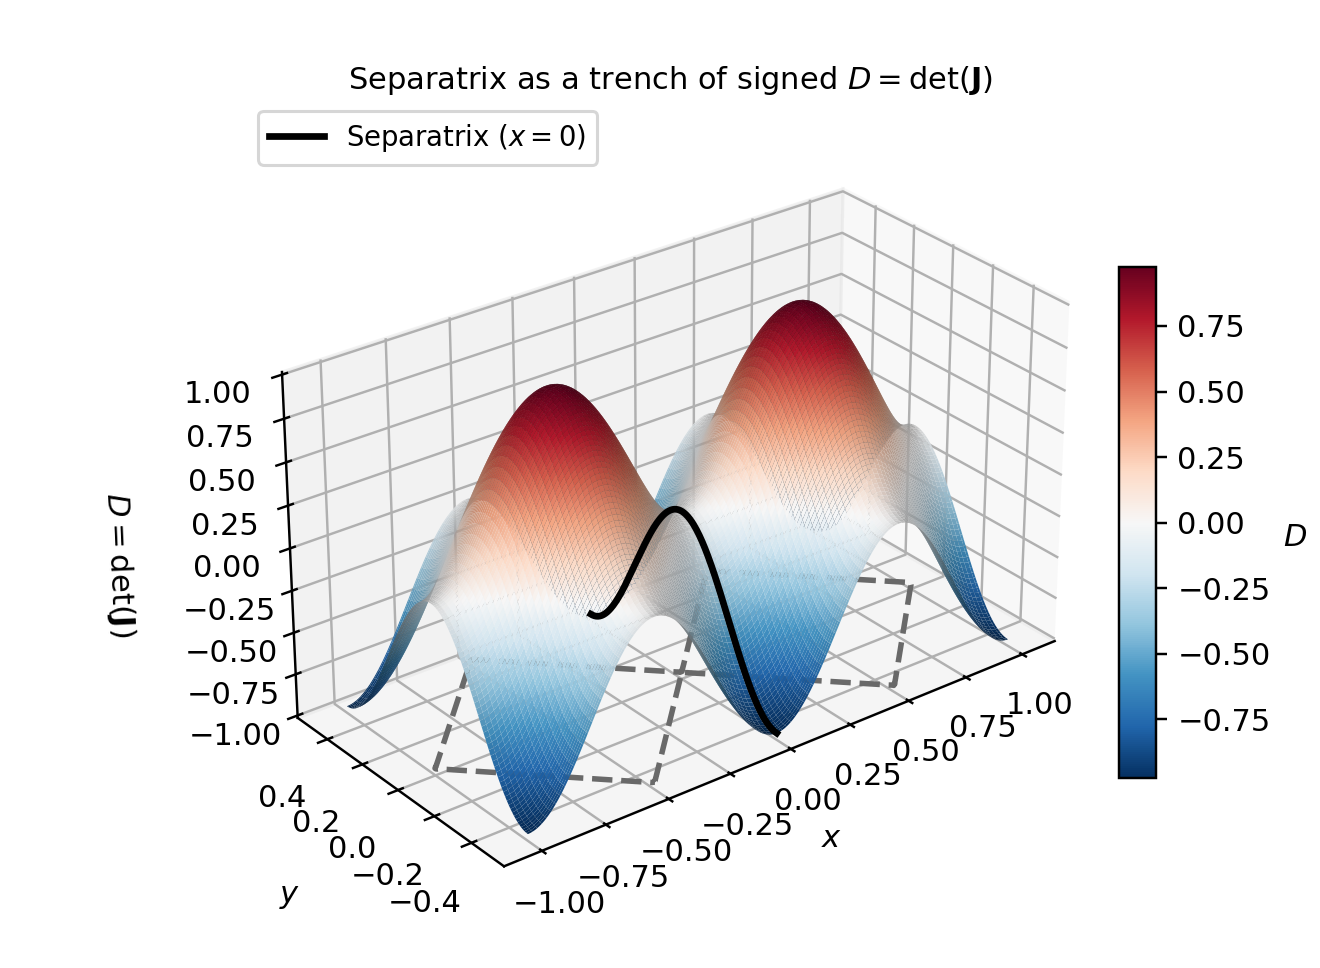
\includegraphics[width=0.36\textwidth]{figures/detJ_trench_cross_section.png}
    \caption{Signed $D$ as an elevation surface over the double gyre.
    The gyre cores rise as ridges ($D > 0$); the separatrix at $x = 0$
    (bold) is a valley of $D$, deepest at the saddles and rising to
    $D = 0$ at the origin.}
    \label{fig:trench_cross}
\end{figure}

\subsection{Problem Statement}
\label{sec:problem_statement}

Consider $N$ robots at positions $\mathbf{p}_i$, each measuring the
local flow $(u_i, v_i) = \mathbf{v}(\mathbf{p}_i)$ at the common
sampling instant, with no map, forecast, or prior field model and no
trajectory integration. The measured flow is a sampled datum, not a
current that advects the platform: robot motion is commanded by the
control law, not advected by the sampled flow. Using
only the current synchronous samples at
each control cycle, the team must generate a centroid velocity command
$\dot{\mathbf{p}}_c$ that solves one of two problems, one per term of
(\ref{eq:splitting}):

\emph{Problem 1 (separatrix network traversal).} Drive the cluster
centroid onto the trench of $D$ and travel it, in the direction of the
ambient flow, through the saddle points where trench segments cross.

\emph{Problem 2 (objective network traversal).} Drive the centroid onto
the trench of $s_1$ and travel it, through the eigenvector swap where the
attracting and repelling segments meet, to a terminal attracting core
where the trench bottoms out, using only objective quantities throughout.


\section{Cooperative Second-Order Estimation}
\label{sec:estimation}

\subsection{Quadratic Fit from Six Simultaneous Measurements}

With robot positions $\mathbf{p}_i = (x_i, y_i)$ again measured from the
centroid, define the quadratic basis vector
\begin{equation}
    \boldsymbol{\phi}(\mathbf{p}) =
    \bigl[\,1, \; x, \; y, \; xy, \;
    \tfrac{1}{2}x^2, \; \tfrac{1}{2}y^2\,\bigr]^\top,
    \label{eq:basis}
\end{equation}
whose entries are the terms of
(\ref{eq:quad_model_u})--(\ref{eq:quad_model_v}) in the same order, so
the recovered coefficients estimate the Taylor derivatives directly with
no rescaling. Stacking the six robots' basis vectors row-wise gives
the $6 \times 6$ formation matrix $\boldsymbol{\Phi}$, and the coefficient
estimates $\hat{\boldsymbol{\theta}}_u = [\hat{a}_1, \ldots,
\hat{a}_6]^\top$ and $\hat{\boldsymbol{\theta}}_v = [\hat{b}_1, \ldots,
\hat{b}_6]^\top$ solve
\begin{equation}
    \boldsymbol{\Phi}\,\hat{\boldsymbol{\theta}}_u = \mathbf{m}_u, \qquad
    \boldsymbol{\Phi}\,\hat{\boldsymbol{\theta}}_v = \mathbf{m}_v,
    \label{eq:solve}
\end{equation}
where $\mathbf{m}_u = [u_1, \ldots, u_6]^\top$ and
$\mathbf{m}_v = [v_1, \ldots, v_6]^\top$ collect the measurements, $u_i$
and $v_i$ being the field components sampled by robot $i$. One matrix
factorization serves both components. If the field is exactly quadratic
over the formation footprint, the $\mathcal{O}(\|\mathbf{p}\|^3)$
remainder vanishes identically, and noise-free measurements give
$\hat{\boldsymbol{\theta}}_u = \boldsymbol{\theta}_u$ and
$\hat{\boldsymbol{\theta}}_v = \boldsymbol{\theta}_v$ for any nonsingular
$\boldsymbol{\Phi}$; neither condition holds exactly in practice.

\begin{proposition}[Minimality]
\label{prop:minimality}
A synchronous sample from fewer than six robots leaves the
unconstrained quadratic model unidentifiable.
\end{proposition}

\begin{IEEEproof}
Each robot contributes one equation per component to (\ref{eq:solve}),
and each system has six unknowns, so fewer than six robots leave the
solution set a positive-dimensional affine subspace.
\end{IEEEproof}

Any method returning a single answer from five robots is therefore
supplying a structural prior rather than reading one from the data. Such
a prior is available: imposing exact incompressibility ties $a_2 + b_3 =
0$ together with its two first derivatives, removing three coefficients,
so five robots then supply ten equations for nine unknowns. The
estimator fits the unconstrained model deliberately, extending to the
constitutive assumption on the field the same refusal to presuppose
that motivates the rest of the method: this paper's approach already
requires neither pre-straddling an assumed manifold nor accumulation of
data points (Section~\ref{sec:intro}), and the sixth robot buys the same
independence from a constitutive assumption about the field, exactness
over every planar quadratic field rather than only over an incompressible
subclass.\label{rem:minimality_priors}

Six robots suffice exactly when $\boldsymbol{\Phi}$ is nonsingular, and
the singular formations admit a clean geometric description.

\begin{proposition}[Conic criterion]
\label{prop:conic}
$\boldsymbol{\Phi}$ is singular if and only if the six sampling points
lie on a common conic, including degenerate conics such as line pairs.
\end{proposition}

\begin{IEEEproof}
$\boldsymbol{\Phi}$ is singular exactly when
$\boldsymbol{\Phi}\mathbf{c} = \mathbf{0}$ for some nonzero
$\mathbf{c} \in \mathbb{R}^6$. Row $i$ of $\boldsymbol{\Phi}$ is
$\boldsymbol{\phi}(\mathbf{p}_i)^\top$, so this holds if and only if
$\boldsymbol{\phi}(\mathbf{p}_i)^\top \mathbf{c} = 0$ for every $i$,
that is, if and only if all six points lie on the zero set of the nonzero
quadratic polynomial $\boldsymbol{\phi}(\cdot)^\top \mathbf{c}$.
\end{IEEEproof}

The criterion carries a practical warning: any six robots on one circle,
a regular hexagon for example, are singular regardless of size or
orientation. Moving one robot to the center removes the degeneracy
entirely.

\begin{corollary}[Pentagon-plus-center]
\label{cor:pentagon}
The pentagon-plus-center formation, five robots on a ring of radius
$\rho$ at $72^\circ$ spacing and one at the center, is nonsingular.
\end{corollary}

\begin{IEEEproof}
A conic vanishing at five points of a circle must be a multiple of that
circle, and a circle does not pass through its own center, so the six
points lie on no common conic.
\end{IEEEproof}

This is the configuration \cite{15} derived for scalar Hessian
estimation, whose
fixed symmetric weights are exact only for the ideal ring geometry and
bias the recovered Hessian under formation deformation. Solving
(\ref{eq:solve}) at the measured positions instead costs one
$6 \times 6$ factorization per cycle, reused for
both components, and stays exact under any deformation short of the
conic degeneracy, with formation error entering only through the
conditioning of $\boldsymbol{\Phi}$ (Section~\mbox{VII-C}).

\subsection{Closed-Form Recovery of $D$, $\nabla D$, and $\mathbf{H}_D$}

The estimated Jacobian at the centroid is assembled from the linear
coefficients,
\begin{equation}
    \hat{\mathbf{J}}_0 =
    \begin{bmatrix}
        \hat{a}_2 & \hat{a}_3 \\ \hat{b}_2 & \hat{b}_3
    \end{bmatrix},
    \qquad
    \hat{D}_0 = \hat{a}_2 \hat{b}_3 - \hat{a}_3 \hat{b}_2.
    \label{eq:J_hat}
\end{equation}
Away from the centroid the fitted model makes every Jacobian entry affine
in position,
\begin{equation}
    \hat{\mathbf{J}}(\mathbf{p}) = \hat{\mathbf{J}}_0 +
    \begin{bmatrix}
        \hat{a}_5 x + \hat{a}_4 y &
        \hat{a}_4 x + \hat{a}_6 y \\
        \hat{b}_5 x + \hat{b}_4 y &
        \hat{b}_4 x + \hat{b}_6 y
    \end{bmatrix},
    \label{eq:jac_affine}
\end{equation}
so $\hat{D}(\mathbf{p}) = \det(\hat{\mathbf{J}}(\mathbf{p}))$ is an exactly
quadratic polynomial in position over the footprint. Differentiating
it and evaluating at the centroid $\mathbf{p} = \mathbf{0}$ gives the
gradient and Hessian there as polynomials in the fitted coefficients:
\begin{equation}
    \hat{\mathbf{g}}_0 =
    \begin{bmatrix}
        \hat{a}_5 \hat{b}_3 + \hat{a}_2 \hat{b}_4
            - \hat{a}_4 \hat{b}_2 - \hat{a}_3 \hat{b}_5 \\
        \hat{a}_4 \hat{b}_3 + \hat{a}_2 \hat{b}_6
            - \hat{a}_6 \hat{b}_2 - \hat{a}_3 \hat{b}_4
    \end{bmatrix},
    \label{eq:grad_det}
\end{equation}
\begin{equation}
    \hat{\mathbf{H}}_{D,0} =
    \begin{bmatrix}
        2(\hat{a}_5 \hat{b}_4 - \hat{a}_4 \hat{b}_5) &
        \hat{a}_5 \hat{b}_6 - \hat{a}_6 \hat{b}_5 \\
        \hat{a}_5 \hat{b}_6 - \hat{a}_6 \hat{b}_5 &
        2(\hat{a}_4 \hat{b}_6 - \hat{a}_6 \hat{b}_4)
    \end{bmatrix}.
    \label{eq:hess_det}
\end{equation}
Because $\hat{D}$ is quadratic, $\hat{\mathbf{H}}_{D,0}$ is independent of
position, the model reports the same curvature everywhere in the
footprint, and unlike the gradient it does not sharpen as the cluster
contracts onto the target.

The two quantities also differ in what the truncation costs them. Every
term of $\nabla D(\mathbf{p}_c)$ pairs a second derivative of the field
with a first derivative, so the quadratic model retains all of the field
data the true gradient depends on. The Hessian does not have that
property. Written in derivatives of the true field, its $(1,1)$ entry
expands as
\begin{equation}
\begin{split}
    D_{xx} = {}&2(u_{xx} v_{xy} - u_{xy} v_{xx}) \\
        &+ u_{xxx} v_y + u_x v_{xxy}
        - u_{xxy} v_x - u_y v_{xxx},
\end{split}
    \label{eq:Dxx_true}
\end{equation}
whose first pair is what (\ref{eq:hess_det}) recovers as $2(\hat{a}_5
\hat{b}_4 - \hat{a}_4 \hat{b}_5)$. The four third-order terms have no
counterpart among the twelve fitted coefficients: they are set to zero by
construction, not made small by a good fit. With the
estimated flow at the centroid, $\hat{\mathbf{v}}_0 = (\hat{a}_1,
\hat{b}_1)$, (\ref{eq:J_hat})--(\ref{eq:hess_det}) supply every quantity
the $D$ tracker consumes.

\subsection{Closed-Form Recovery of $s_1$ and the Strain Eigenframe}
\label{sec:s1_estimation}

The same fit supplies the objective strain quantities. Write $\mu$,
$s_n$, and $s_s$ for the
mean, deviatoric normal, and shear strain, which the fitted first-order
coefficients give as
\begin{equation}
    \mu = \frac{\hat{a}_2 + \hat{b}_3}{2}, \quad
    s_n = \frac{\hat{a}_2 - \hat{b}_3}{2}, \quad
    s_s = \frac{\hat{a}_3 + \hat{b}_2}{2},
    \label{eq:strain_parts}
\end{equation}
with $\mu = 0$ for incompressible flow. The strain eigenvalues are
$s_{1,2} = \mu \mp r$ with $r = \sqrt{s_n^2 + s_s^2}$, and the
eigenframe $(\mathbf{e}_1, \mathbf{e}_2)$ is that of the symmetric
matrix $\hat{\mathbf{S}}$ assembled from the same coefficients. Under
the quadratic model, $\mu$, $s_n$, and $s_s$ are affine functions of
position, so the gradient of $\hat{s}_1$ is exact for the fitted field:
\begin{equation}
    \nabla \hat{s}_1 = \nabla\mu
    - \frac{s_n\,\nabla s_n + s_s\,\nabla s_s}{r},
    \label{eq:grad_s1}
\end{equation}
with $\nabla\mu$, $\nabla s_n$, $\nabla s_s$ read directly off the
second-order coefficients (for example $\nabla s_n = \tfrac{1}{2}
(\hat{a}_5 - \hat{b}_4,\; \hat{a}_4 - \hat{b}_6)^\top$). Two properties
distinguish this pipeline from the $D$ pipeline, one favorable and one
prohibitive.

The favorable one: the tangent the $s_1$ tracker rides,
$\mathbf{e}_2$, comes from the \emph{first-order} fitted coefficients,
one derivative order better in noise gain than the
$\hat{\mathbf{H}}_D$ eigenvectors the $D$ tracker uses for the same
purpose, and free of the floor those eigenvectors carry
(Table~\ref{tab:budget}).

\begin{remark}[No usable Hessian of $s_1$ exists under a quadratic fit]
\label{rem:s1hess}
The prohibitive one: a Newton step on $(\nabla \hat{s}_1,
\hat{\mathbf{H}}_{s_1})$ is impossible in principle, not merely
inaccurate. Under the quadratic model the map $\mathbf{p} \mapsto (s_n,
s_s)$ is affine, so $\hat{s}_1 = \mu - \|(s_n, s_s)\|$ is concave and its
Hessian is negative semidefinite \emph{for every field and every
formation}; the positive transverse curvature of an $s_1$ trench lives
in third derivatives of the velocity field, outside the span of any
quadratic fit. (On the double gyre, where $s_s \equiv 0$, the fitted
$\hat{\mathbf{H}}_{s_1}$ is numerically zero.) The gradient
(\ref{eq:grad_s1}) is unaffected: its transverse component recovers the
trench-restoring signal with the correct sign.
\end{remark}

\subsection{Estimator Sensitivity}
\label{sec:sensitivity}

Two channels perturb the samples. Measurement noise is additive
Gaussian on the components each robot reads,
\begin{equation}
    u_i^m = u(\mathbf{p}_i) + \eta_i^u, \quad
    v_i^m = v(\mathbf{p}_i) + \eta_i^v,
    \quad \eta \sim \mathcal{N}(0, \sigma_{uv}^2),
    \label{eq:meas_noise}
\end{equation}
independent across robots, components, and steps, the sensor model of
\cite{9}. Position noise perturbs where each robot
samples,
\begin{equation}
    (u_i^m, v_i^m) = \mathbf{v}(\mathbf{p}_i + \boldsymbol{\xi}_i), \quad
    \boldsymbol{\xi}_i \sim \mathcal{N}(\mathbf{0}, \sigma_p^2 \mathbf{I}),
    \label{eq:pos_noise}
\end{equation}
while the fit (\ref{eq:solve}) uses the nominal $\mathbf{p}_i$. A
displaced robot commits the reading error
$\mathbf{J}\boldsymbol{\xi}_i$ to first order, so the two channels
combine into one effective level,
\begin{equation}
    \sigma_{\mathrm{eff}}^2 = \sigma_{uv}^2
        + \tfrac{1}{2}\lVert\mathbf{J}\rVert_F^2\,\sigma_p^2 .
    \label{eq:sigma_eff}
\end{equation}

The fit is linear, so $\hat{\boldsymbol{\theta}} -
\boldsymbol{\theta} = \boldsymbol{\Phi}^{-1}\boldsymbol{\eta}$ exactly
and the analysis is a calculation of row norms. For the
pentagon-plus-center, a coefficient of derivative order $q$ has
\begin{equation}
    \sigma_{\theta_q} = \gamma_q\,
    \frac{\sigma_{\mathrm{eff}}}{\rho^{\,q}},
    \qquad
    \gamma_0 = 1, \;\;
    \gamma_1 = \tfrac{2}{\sqrt{10}}, \;\;
    \gamma_2 = \tfrac{8}{\sqrt{10}},
    \label{eq:gain_ladder}
\end{equation}
with $\gamma_2 = 4/\sqrt{10}$ for the mixed coefficients and gradient
covariance $\tfrac{4}{10}\sigma_{\mathrm{eff}}^2\rho^{-2}\mathbf{I}$,
isotropic at every heading (Appendix~\ref{app:proofs}). Only $\gamma_q$ is specific to this
formation; the exponent is not, since order $q$ costs $q$ difference
quotients and only the signal scales with $\rho$. An affine fit returns
no second derivatives at all: three robots locate a critical point
\cite{14}, six supply the curvature and eigenframe the trackers
consume.

Truncation pulls the other way. With $U$ and $L$ the velocity and length
scales of the field, form
\begin{equation}
    \nu = \frac{\sigma_{\mathrm{eff}}}{U}, \qquad
    \tilde{\rho} = \frac{\rho}{L}.
    \label{eq:groups}
\end{equation}
A quantity of order $q$ has magnitude $U/L^{\,q}$, so its relative noise
error is $\nu/\tilde{\rho}^{\,q}$, while the discarded term of order
$p+1$ biases it by a relative $\tilde{\rho}^{\,p+1-q}$:
\begin{equation}
    E_q(\tilde{\rho}) = c\,\frac{\nu}{\tilde{\rho}^{\,q}}
        + d\,\tilde{\rho}^{\,p+1-q}.
    \label{eq:error_budget}
\end{equation}
The exponents sum to $p+1$ by construction, noise counting the orders
extracted and truncation the orders remaining, so $\tilde{\rho}^*
\propto \nu^{1/(p+1)}$, a cube root here. The optimum differs between
$\hat{D}$ and $\nabla\hat{D}$, and neither constant is computable in the
field: $\rho$ is fixed at $0.075$ on the double gyre and set by the sampling requirement of
Section~\mbox{V-C} on the ocean field.

Two terms escape (\ref{eq:error_budget}), each adding a constant. Some
quantities need derivatives the model does not carry:
(\ref{eq:Dxx_true}) splits into a fitted pair and four third-order terms
of the same size as $D_{xx}$ itself, set to zero by construction rather
than made small by a good fit, contributing a floor $e = O(1)$
independent of $\rho$, $\sigma_{\mathrm{eff}}$, and formation.
The same audit of $\nabla D$ returns nothing, every term of it pairing a
fitted second derivative with a fitted first, so any measured gap
between the two is $e$ alone. The floor destroys sign information where
an eigenvalue crosses zero but leaves directions usable, so
$\hat{\mathbf{H}}_D$ can steer a controller and cannot tell it when to
stop. The second constant
is the observer: a rotation at $\Omega$ is absorbed by the spin part and
not the strain part, so (\ref{eq:D_not_objective}) contaminates every
determinant-derived quantity by a relative $O(\mathrm{Ro})$,
$\mathrm{Ro} = \Omega L/U$, again with no $\nu$, $\tilde{\rho}$, or
formation geometry in it.

Both surrogates sit on the same rung, and what separates them is
algebraic. $D$ is a quadratic form in the first-order coefficients,
while $s_1 = \mu - r$ is a norm subtracted from an affine function. A
perturbed norm projects the noise onto a unit vector, so $\sigma_{s_1} =
\gamma_1\sigma_{\mathrm{eff}}/\rho$ however poorly the eigenframe is
resolved; the eigenframe divides by that magnitude instead, and its
angular error carries an extra $1/r$.

\begin{table}[!t]
\centering
\caption{Error budget by channel. $\nu$ and $\tilde{\rho}$ are the
relative noise and radius of (\ref{eq:groups}), $e$ the
unmodelled-derivative floor, $\mathrm{Ro}$ the observer term, and $r$
the deviatoric strain magnitude of Section~\mbox{III-C}.
$\hat{\mathbf{H}}_D$ is at once the only curvature available to either
tracker and the only quantity either consumes that carries a floor.}
\label{tab:budget}
\footnotesize
\setlength{\tabcolsep}{4pt}
\begin{tabular}{@{}lccccc@{}}
\hline
quantity & noise & trunc. & floor & frame & gap \\
\hline
$\hat{D}$ & $\nu/\tilde{\rho}$ & $\tilde{\rho}^2$ & --- & $O(\mathrm{Ro})$ & --- \\
$\hat{s}_1$ & $\nu/\tilde{\rho}$ & $\tilde{\rho}^2$ & --- & --- & --- \\
$\nabla\hat{D}$ & $\nu/\tilde{\rho}^2$ & $\tilde{\rho}$ & --- & $O(\mathrm{Ro})$ & --- \\
$\nabla\hat{s}_1$ & $\nu/\tilde{\rho}^2$ & $\tilde{\rho}$ & --- & --- & --- \\
$\hat{\mathbf{H}}_D$ eigenvalues & $\nu/\tilde{\rho}^2$ & $\tilde{\rho}$ & $e = O(1)$ & $O(\mathrm{Ro})$ & --- \\
strain eigenframe & $\nu/\tilde{\rho}$ & $\tilde{\rho}^2$ & --- & --- & $\div\,r$ \\
$\hat{\mathbf{H}}_{s_1}$ & --- & --- & sign wrong & --- & undef. at $r=0$ \\
\hline
\end{tabular}
\end{table}

\begin{figure}[!t]
    \centering
    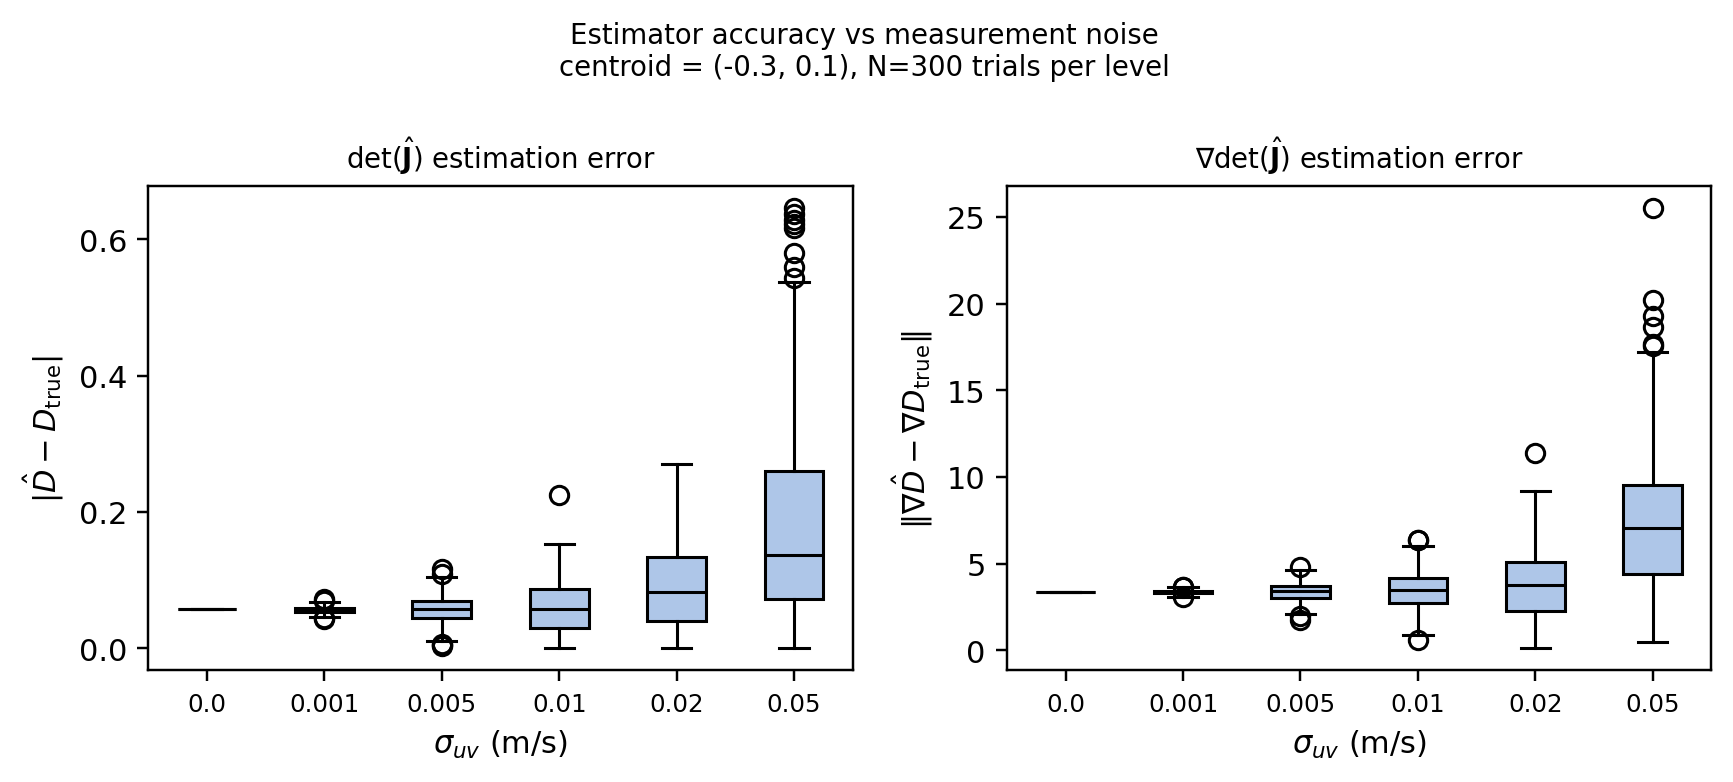
\includegraphics[width=0.34\textwidth]{figures/estimator_accuracy_vs_noise.png}
    \caption{Relative estimation error of $\hat{D}$, $\nabla\hat{D}$, and
    $\hat{\mathbf{H}}_D$ on the steady double gyre (median over $2 \times
    10^5$ noise draws per point; the dashed line marks error equal to
    signal). (a) Versus measurement noise at $\rho = 0.075$; the
    dash-dotted line marks the noise level where closed-loop traverse
    success crosses 50\% (Table~\ref{tab:mc_success}). (b) Versus
    formation radius at $\sigma_{uv} = 0.01$; dotted curves are the
    noise-free truncation floors. On these axes the exponents of
    (\ref{eq:error_budget}) appear as slopes.}
    \label{fig:est_accuracy}
\end{figure}

Over $2\times10^5$ draws per condition at a static strain-region point
of the double gyre, every coefficient standard deviation matched (\ref{eq:gain_ladder}) within 0.3\% and the position-noise
reading error matched (\ref{eq:sigma_eff}) within 1.1\%. In
Fig.~\ref{fig:est_accuracy}(a), $\hat{D}$ stays informative to
$\sigma_{uv} \approx 0.06$ and $\nabla\hat{D}$ to $\approx 0.01$, while
$\hat{\mathbf{H}}_D$ sits at the error-equals-signal line even for the
quietest sensors, held there by $e$; its eigendirections remain accurate
to $0.35^\circ$ near the separatrix and $3.8^\circ$ at a generic point,
the eigenvalues absorbing the floor. Closed-loop
degradation should therefore begin near $\sigma_{uv} = 0.01$.

\section{Adaptive Navigation Controllers}
\label{sec:controllers}

This section derives the two controllers. They share the estimation
step, the saturation idiom, and the three-layer architecture below.
Every difference between them follows from which term of
(\ref{eq:splitting}) the tracker uses: both, for the $D$ tracker's
network reach; the strain term alone, for the $s_1$ tracker's frame
invariance.

\subsection{Multilayer Control Architecture}
\label{sec:arch}

The trackers run inside the layered control architecture of prior
cluster space control studies \cite{14,28,27,30}, shown in
Fig.~\ref{fig:control_architecture}. The adaptive navigation layer is
the only one that reads the field: each cycle it takes the six
synchronous position and velocity-field measurements (a separate
channel from robot actuation, per the modelling assumption of
Section~\mbox{II-E}), recovers the estimated field quantities, applies
whichever tracker's control law
is active, and passes the desired centroid
velocity down. The cluster space layer holds the formation rigid
around that centroid command using a cluster-of-clusters
parameterization, robots grouped into three pairs (length $L$, angle
$\theta$ each) whose midpoints form a Side-Angle-Side triangle
\cite{31}, twelve cluster variables in place of the twelve Cartesian
coordinates, nine of them shape, regulated to the pentagon-plus-center nominal
(Corollary~\ref{cor:pentagon}) except the centroid and heading, which
the top layer's command alone determines. The adaptive navigation layer
is where the two trackers of this paper actually differ from each other: everything
beneath it is a fixed, tracker-agnostic mechanism, so replacing the $D$
tracker with the $s_1$ tracker changes nothing about the two layers
beneath it.

\begin{figure}[!t]
    \centering
    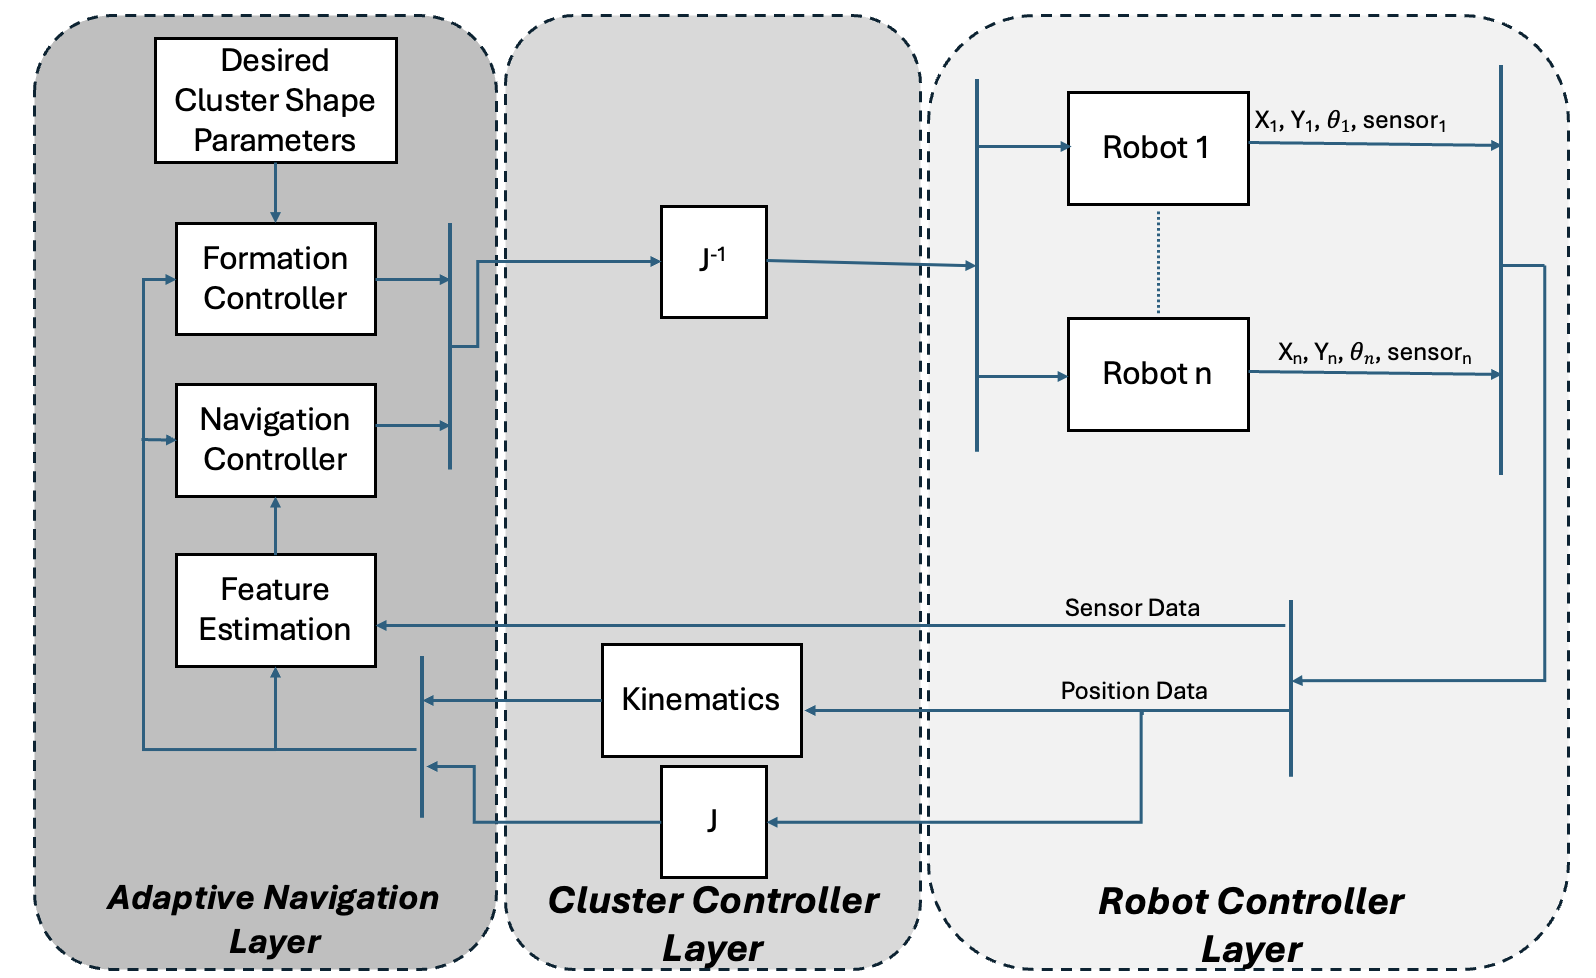
\includegraphics[width=0.40\textwidth]{figures/control_architecture.png}
    \caption{Hierarchical control architecture: robot, cluster space,
    and adaptive navigation layers.}
    \label{fig:control_architecture}
\end{figure}


\subsection{The $D$ Tracker}
\label{sec:sep_controller}

The $D$ tracker drives the cluster centroid onto the trench of $D$ and
then along it, following the separatrix through the crest that separates
one saddle from the next: this is Problem 1. Both motions are built from
the local quadratic surface the estimator returns.

We work in the eigenbasis of the estimated Hessian. Let
$\hat{\mathbf{H}}_{D,0}\mathbf{w}_k = \lambda_k \mathbf{w}_k$ with
$\|\mathbf{w}_k\| = 1$ and $\lambda_1 \leq \lambda_2$. A trench of $D$ is
convex across and concave along, so it is the case
$\lambda_1 < 0 < \lambda_2$: the eigenvector $\mathbf{w}_2$ points across
the trench and $\mathbf{w}_1$ points along it. The sign of an eigenvector
is arbitrary, and we fix the sign of $\mathbf{w}_1$ so that
$\hat{\mathbf{v}}_0^\top \mathbf{w}_1 \geq 0$, which orients it
downstream.

Because $\hat{D}$ is an exact quadratic surface, the Newton step
$-\hat{\mathbf{H}}_{D,0}^{-1}\hat{\mathbf{g}}_0$ moves in one stroke to
its stationary point. Two properties prevent us from issuing it as a
velocity command. Its magnitude grows without bound as
$\hat{\mathbf{H}}_{D,0}$ approaches singularity, and the stationary point
it seeks is the crest of the trench rather than a point on the
separatrix. We bound the first with the saturation
\begin{equation}
    \mathrm{sat}(c) = c_{\max} \tanh\!\left(\frac{c}{c_{\max}}\right),
    \label{eq:sat}
\end{equation}
and address the second by treating the two eigendirections separately.

Across the trench, the Newton component is what we want, and we keep it.
Along the trench, we keep its magnitude and take its direction from the
ambient flow, which is what distinguishes the separatrix we are
following from the crest we are passing through.

The along-trench command changes character once the cluster reaches the
separatrix. Away from it, the along-trench gradient supplies a descent
rate. On it, that gradient vanishes at the crest and the descent rate
vanishes with it, while the separatrix continues through, so the flow
supplies the speed instead. We declare the cluster on the separatrix,
written $\mathbf{p}_c \in \mathcal{B}$, when
\begin{equation}
    |\hat{D}_0| < \varepsilon_{\mathrm{raw}}
    \quad\text{or}\quad
    \frac{|\hat{D}_0|}{\|\hat{\mathbf{H}}_{D,0}\|_F}
        < \varepsilon_{\dim}.
    \label{eq:flow_band}
\end{equation}
The first test is a raw threshold on the estimated determinant. The
second normalizes it by the local curvature, so that the band scales
with the landscape rather than with the absolute size of $D$; the ratio
has units of length squared, which fixes the band width in physical
units. The along-trench speed is then
\begin{equation}
    \tau =
    \begin{cases}
        \hat{\mathbf{v}}_0^\top \mathbf{w}_1,
            & \mathbf{p}_c \in \mathcal{B}, \\[6pt]
        \dfrac{|\mathbf{w}_1^\top \hat{\mathbf{g}}_0|}{|\lambda_1|},
            & \text{otherwise},
    \end{cases}
    \label{eq:tau}
\end{equation}
and the velocity command is
\begin{equation}
    \dot{\mathbf{p}}_c =
    \mathrm{sat}(\tau)\,\mathbf{w}_1
    + \mathrm{sat}\!\left(-\frac{\mathbf{w}_2^\top
      \hat{\mathbf{g}}_0}{\lambda_2}\right)\mathbf{w}_2.
    \label{eq:d_law}
\end{equation}

This control law decouples transverse and tangential motion. The
$\mathbf{w}_2$ term is unaffected by (\ref{eq:tau}) and is therefore the
same command on and off the band. It snaps the centroid onto the trench
floor, and recovers the exact Newton component, with its superlinear
local convergence, once the argument falls inside the boundary layer.
The $\mathbf{w}_1$ term carries the centroid along the structure at the
curvature-normalized rate off the band and at the flow speed on it.
Since $\tau \geq 0$ in both cases, the tangential motion is never
directed against the ambient flow. The single parameter $c_{\max}$ sets
the cruise speed far from the structure and the width of the terminal
boundary layer near it.

The trench frame is undefined when $\hat{\mathbf{H}}_{D,0}$ has
eigenvalues of one sign, so (\ref{eq:d_law}) needs a fallback there:
off the band it reverts to the signed Newton step $\sum_k
\mathrm{sat}(-\mathbf{w}_k^\top\hat{\mathbf{g}}_0/\lambda_k)\mathbf{w}_k$,
which drives the centroid toward the nearest stationary point of
$\hat{D}$ without a stability claim, and on the band it reverts to the
saturated flow alone; with exact estimates, neither case arises on a
trench away from the band boundary.

Finally, the command is well defined despite the sign ambiguity of
eigenvectors. The transverse term is quadratic in $\mathbf{w}_2$ and so
does not depend on its sign, and the tangential term fixes the sign of
$\mathbf{w}_1$ explicitly.


\subsection{The $s_1$ Tracker}
\label{sec:oecs_controller}

The strain eigenvalue $s_1$ is objective where $D$ is not. The second
controller solves Problem 2, testing whether that guarantee is
reachable with the same cooperative, map-free, single-sample estimator,
riding the separatrix network rather than a bounded segment of it.

The controller traverses the trench of $s_1$ using four quantities the
fit delivers: the eigenvalue $\hat{s}_1$, its gradient
$\nabla\hat{s}_1$, the strain eigenframe $(\mathbf{e}_1, \mathbf{e}_2)$,
and the deviatoric strain magnitude $r$, which is half the eigenvalue gap
and therefore measures how well resolved that eigenframe is.
Remark~\ref{rem:s1hess} rules out a Newton snap on $s_1$, so both
channels of this controller are built from the gradient rather than the
curvature.

We first identify the trench tangent. Naming an eigenvector directly will
not work, because which of the two is tangent swaps at the degeneracy
lines. Instead we use the gradient. On the trench, the transverse
derivative of $s_1$ vanishes by construction, so away from a stationary
point $\nabla\hat{s}_1$ points almost entirely along the trench, and the
tangent is whichever eigenvector the gradient is less orthogonal to:
\begin{equation}
    \mathbf{t}_{\mathrm{raw}} =
    \arg\max_{\mathbf{e} \in \{\mathbf{e}_1, \mathbf{e}_2\}}
    \bigl\lvert \nabla\hat{s}_1^\top \mathbf{e} \bigr\rvert,
    \qquad
    \mathbf{t} = \mathrm{sgn}\bigl(\mathbf{t}_{\mathrm{ref}}^\top
    \mathbf{t}_{\mathrm{raw}}\bigr)\,\mathbf{t}_{\mathrm{raw}},
    \label{eq:tangent_select}
\end{equation}
where $\mathbf{t}_{\mathrm{ref}}$ is the previous step's tangent once one
has been established, or the measured flow $\hat{\mathbf{v}}_0$ on the
first tracking step. This rule selects $\mathbf{e}_2$ on the attracting
half of the separatrix and $\mathbf{e}_1$ on the repelling half, swapping
automatically through the origin. The same comparison resolves which
branch to continue onto at a network crossing, where the wall trench has
its own, larger projection. Continuity fixes only the residual sign; the
direction itself does not depend on it.

The controller alternates between two behaviors. While traversing, it
rides along $\mathbf{t}$ at constant speed and descends $\hat{s}_1$ only
across the trench. While settling, it stops riding and descends
$\hat{s}_1$ in every direction. Let $\beta \in \{0,1\}$ be the ride flag,
one while traversing and zero while settling. The velocity command is
\begin{equation}
    \dot{\mathbf{p}}_c =
    \beta\,c_{\max}\tanh(1)\,\mathbf{t}
    - \mathrm{sat}\!\bigl(g_\perp\,\mathbf{P}\,\nabla\hat{s}_1\bigr),
    \qquad
    \mathbf{P} = \mathbf{I} - \beta\,\mathbf{t}\mathbf{t}^\top,
    \label{eq:oecs_law}
\end{equation}
where $\mathrm{sat}$ acts on a vector by saturating its magnitude and
preserving its direction, reducing to (\ref{eq:sat}) on any scalar
multiple of a unit vector.

This control law decouples descent from travel through the projector.
With $\beta = 1$, $\mathbf{P}$ removes the along-trench component of the
gradient, so the team descends only across the trench while riding along
it at cruise speed $c_{\max}\tanh(1)$. With $\beta = 0$, the projector
becomes the identity, the ride term drops out, and the same expression
is full gradient descent on $\hat{s}_1$, which settles at a local
minimum. The gain $g_\perp$ is fixed, standing in for the curvature
normalization that Remark~\ref{rem:s1hess} rules out, so the transverse
channel contracts at gradient rate rather than at Newton rate. This is
the first cost of objectivity. Both channels read the same two
projections from (\ref{eq:tangent_select}), so no additional estimated
quantity enters the ride.

Two situations clear the ride flag. Before the team has reached any
structure, $\beta = 0$ and the descent term homes onto the trench from
anywhere in the basin. We declare first contact, and latch $\beta$ to
one, when $\hat{s}_1$ first falls below $-s_{\mathrm{trim}}$. The second
situation is the terminal behavior, and it holds the team at a
two-dimensional stationary point of $\hat{s}_1$ when
\begin{equation}
    r > r_{\mathrm{band}}, \qquad
    \lVert\nabla\hat{s}_1\rVert < g_{\mathrm{capture}}, \qquad
    \hat{s}_1 < -4 s_{\mathrm{trim}}.
    \label{eq:capture_test}
\end{equation}

A flow saddle is not merely a crossing of two transverse trenches. It is
a genuine two-dimensional minimum of $s_1$, verified numerically at the
double-gyre saddle, so the full gradient collapses there, while at an
ordinary trench point the gradient remains large along the trench even
though it vanishes across it. Testing the gradient magnitude is
therefore enough to distinguish the two. This matters because the
ambient flow also stagnates at a saddle, which would starve any
flow-based tangent rule of a direction exactly where the ride needs one.
The three tests in (\ref{eq:capture_test}) reject, in order, the
isotropic point, an ordinary trench point, and a shallow flat spot of
$\hat{s}_1$ away from real structure. The $-4s_{\mathrm{trim}}$ depth
threshold is a hysteresis ratio, not a physical relation: the test arms
at four times the first-contact depth and releases at one times it, so
noise near the contact level cannot arm and disarm the test on
successive steps. The condition latches once
satisfied and releases when $\hat{s}_1$ rises back above
$-s_{\mathrm{trim}}$, the same threshold that declares first contact. A
noise-driven flicker of the gradient test therefore does not send the
team back through the tangent comparison at the well, while a genuine
departure from the well still does.

One guard falls outside (\ref{eq:oecs_law}). If the eigenframe is
degenerate, $r < r_{\mathrm{band}}$, and no previous tangent has been
established, then neither (\ref{eq:tangent_select}) nor continuity
supplies a direction. The command then rides the measured flow,
$\mathbf{t} = \hat{\mathbf{v}}_0/\|\hat{\mathbf{v}}_0\|$, with the
projector set to the identity. Only the first tracking step can reach
this case, and it is the one place in the controller where the ambient
flow enters the command.



\subsection{Stability Properties}
\label{sec:stability}

The analysis is at the navigation level, with the cluster centroid a
kinematic integrator
\begin{equation}
    \dot{\mathbf{p}}_c = k\,\boldsymbol{\delta}(\mathbf{p}_c),
    \label{eq:kinematic_model}
\end{equation}
$\boldsymbol{\delta}$ the right-hand side of the active law,
(\ref{eq:d_law}) or (\ref{eq:oecs_law}), and $k > 0$ the navigation
gain. This abstracts the layers beneath, whose dynamics settle in
roughly 0.3~s against transit times of tens of seconds \cite{14}.
Estimates are taken exact, so hats are dropped; proofs are in
Appendix~\ref{app:proofs}.

\begin{assumption}[Trench and flow structure]
\label{ass:trench}
Let $\Sigma$ be the tracked surrogate, $D$ or $s_1$. On a tube $T_w =
\{|n| \leq w\}$ about a segment $\Gamma$, in arclength coordinates
$(\ell, n)$ along and across it,
\begin{equation}
    \Sigma(\ell, n) = h(\ell)
        + \tfrac{1}{2}\kappa_\perp(\ell)\,n^2,
    \qquad 0 < \underline{\kappa} \leq \kappa_\perp(\ell),
    \label{eq:normal_form}
\end{equation}
with vanishing cross terms. The curve $\Gamma$ is invariant under the
flow, with $\lVert\mathbf{v}\rVert \geq f_{\min} > 0$ outside balls of
radius $r_0$ around the flow saddles, and $|h'(\ell)| \geq m_h > 0$
wherever the band test fails on $\Gamma$.
\end{assumption}

The transverse gradient $\kappa_\perp n$ vanishes on $\Gamma$ and
nowhere else in the tube, so the problem splits: regulate $n$ to zero,
transport along $\ell$.

The two controllers are the same machine with one number changed. Both
command the transverse law
\begin{equation}
    \dot{n} = -c_{\max}\tanh\!\left(
        \frac{a_\perp\,n}{c_{\max}}\right),
    \label{eq:n_dynamics}
\end{equation}
and differ only in $a_\perp$. The $D$ tracker normalizes by the
estimated curvature, giving the Newton argument $-\kappa_\perp
n/\kappa_\perp = -n$; the $s_1$ tracker has no usable curvature
(Remark~\ref{rem:s1hess}) and substitutes the fixed gain $g_\perp$:
\begin{equation}
    a_{\perp,D} = 1,
    \qquad
    a_{\perp,s_1} = g_\perp\,\kappa_\perp(\ell).
    \label{eq:transverse_rates}
\end{equation}
One rate is fixed by design, the other set by the field.

Two regimes live inside (\ref{eq:n_dynamics}): far out $\tanh$ saturates
into a constant approach at $c_{\max}$, close in it is linear and the
command is proportional, with crossover at $|n| = c_{\max}/a_\perp$.
With $V = \tfrac{1}{2}n^2$, $\dot{V} = -c_{\max}\,n\tanh(a_\perp
n/c_{\max}) < 0$ for $n \neq 0$, so $T_w$ is forward invariant, the
proportional region is entered in finite time, and inside it concavity
of $\tanh$ gives $\dot{V} \leq -2a_\perp\tanh(1)V$.

Once $n \approx 0$ the tangential command takes over, with $\tau \geq 0$
in every branch of (\ref{eq:tau}), leaving one-dimensional transport in
the flow direction. The two phases do not interfere, and the reason is
visible in the law rather than in the analysis: \emph{the transverse
command contains no $\tau$}. The tangential mode switch is therefore
invisible to the regulated variable and cannot move the team across the
structure, and the $s_1$ tracker's projector enforces the same
separation explicitly.

\begin{theorem}[Network traversal]
\label{thm:separatrix}
Under Assumption~\ref{ass:trench}, with exact estimates, every
trajectory starting in $T_w$ (i) remains in $T_w$ and converges
exponentially to $\Gamma$, and (ii) traverses $\Gamma$ in the direction
of the ambient flow, reaching the $r_0$ neighborhood of a flow saddle in
finite time bounded by $L_\Gamma/m$, with $L_\Gamma$ the length of
$\Gamma$ and $m > 0$ the realized tangential speed.
\end{theorem}

At a flow saddle $D$ has a local minimum with $\mathbf{H}_D \succ 0$ and
the degenerate case of (\ref{eq:d_law}) is active. In practice the $D$
tracker continues past it: the floor $e$ of Section~\mbox{III-D} leaves
the estimated eigenvalues indefinite and an order of magnitude too small
there even without noise, so the tracker rides onto the crossing segment
and repeats (i) and (ii) with $\Gamma$ relabeled. Both behaviors are the
same theorem on different premises.

Termination carries its own certificate. When the ride flag clears the
projector becomes the identity and (\ref{eq:oecs_law}) is full gradient
descent on the surrogate itself,
\begin{equation}
    \dot{s}_1 = -c_{\max}\lVert\nabla s_1\rVert
    \tanh\!\left(\frac{g_\perp\lVert\nabla s_1\rVert}{c_{\max}}\right)
    \;\leq\; 0,
    \label{eq:s1_lyapunov}
\end{equation}
with equality only at a critical point: nothing holds the team in place,
it has arrived. This is the vanishing-gradient test
Section~\mbox{III-D} admits rather than the definiteness test it does
not.

Estimation error, and any residual cross term $\kappa_\perp'(\ell)\,n$,
enters the transverse channel as a bounded disturbance $|d| \leq
\delta$. Then $\dot{V} < 0$ outside an interval, and the structure is
practically stable with
\begin{equation}
    \limsup_{t\to\infty}|n(t)| \;\leq\;
    \frac{c_{\max}}{a_\perp}
    \operatorname{artanh}\!\left(\frac{\delta}{c_{\max}}\right)
    \;\approx\; \frac{\delta}{a_\perp},
    \qquad \delta \ll c_{\max},
    \label{eq:iss_bound}
\end{equation}
the disturbance divided by the local slope of the restoring law, which
is why $a_\perp$ matters. Here $\delta$ is the transverse gradient
error, placed at $\nu/\tilde{\rho}^{\,2}$ by Table~\ref{tab:budget}, so
tracking error degrades linearly in measurement noise: no control law
changes that exponent, and only $a_\perp$ scales the result.

\begin{proposition}[Frame equivariance of the closed loop]
\label{prop:equivariance}
Let an observer rotate as $\mathbf{p}_Q = \mathbf{Q}(t)\mathbf{p}$ and
let the $s_1$ tracker run with exact estimates on the correspondingly
transformed field. Then $\boldsymbol{\delta}_Q =
\mathbf{Q}\boldsymbol{\delta}$ and $\mathbf{p}_{c,Q}(t) =
\mathbf{Q}(t)\mathbf{p}_c(t)$ up to the frame-transport term: the
tracker follows the same material path in every frame. The single
exception is the degenerate guard, reachable only on the first tracking
step.
\end{proposition}

Every quantity (\ref{eq:oecs_law}) consumes is invariant or co-rotating,
the tangent selection (\ref{eq:tangent_select}) included. The $D$
tracker admits no counterpart: its surrogate carries the
$O(\mathrm{Ro})$ term of Section~\mbox{III-D} into everything its law
reads.

Two bandwidth limits sit underneath all of this. Explicit Euler at step
$\Delta t$ makes the near-structure map $n \mapsto n(1 - \Delta t\,k\,
a_\perp)$: monotone below $\Delta t\,k\,a_\perp = 1$, stable below $2$,
admitting a limit cycle above it. The kinematic abstraction separately
needs $k\,a_\perp\tau_{\mathrm{mom}} \ll 1$, since a proportional region
narrower than the plant can follow is not a proportional region. Both
read off $a_\perp$ alone, and at the operating point of
Table~\ref{tab:params} they bind for one tracker only.

\begin{table}[!t]
\centering
\caption{Discrete-time and actuator conditions at the double-gyre
operating point of Table~\ref{tab:params} ($\Delta t = 0.1$, $k = 3.0$,
$\tau_{\mathrm{mom}} = 0.28$, $g_\perp = 1.0$). For the $s_1$ tracker
$\kappa_\perp$ is the local transverse curvature of the structure,
quoted as recovered by the fit and as computed analytically at the same
point (Section~\mbox{VI-B-3}).}
\label{tab:bandwidth}
\footnotesize
\setlength{\tabcolsep}{4pt}
\begin{tabular}{@{}lcccl@{}}
\hline
 & $a_\perp$ & $\Delta t\,k\,a_\perp$ &
 $k\,a_\perp\tau_{\mathrm{mom}}$ & \\
\hline
$D$ tracker & $1.0$ & $0.30$ & $0.84$ & monotone \\
$s_1$, fitted $\kappa_\perp = 4.0$ & $4.0$ & $1.20$ & $3.4$ & oscillatory \\
$s_1$, analytic $\kappa_\perp = 6.9$ & $6.9$ & $2.07$ & $5.8$ & limit cycle \\
\hline
\end{tabular}
\end{table}

Two consequences follow. The $s_1$ tracker's larger zero-noise tracking
error is more likely a discretization effect than an estimation one,
since (\ref{eq:iss_bound}) predicts the opposite ranking: a larger
$a_\perp$ gives a \emph{tighter} ultimate bound under equal disturbance,
and only a limit cycle explains a larger error where that bound cannot.
And the loop is stable at the fitted curvature but not at the true one,
so the estimator's underestimate of $\kappa_\perp$ is carrying the
margin. Halving $\Delta t$ separates the two in one run, shrinking a
limit cycle and leaving an estimation error untouched, with the $D$
tracker indifferent either way at $\Delta t\,k\,a_\perp = 0.3$.

\section{Simulation Program}
\label{sec:methods}

\subsection{Simulation Setup}

A Python simulation implementing the three-layer architecture of
Section~\mbox{IV-A} was developed to evaluate both trackers.
The double-gyre experiments use the steady field of
Section~\mbox{II-D} ($A = 0.1$) on the domain $[-1, 1] \times
[-0.5, 0.5]$. The integrator is explicit Euler at 10~Hz ($\Delta t =
0.1$~s), robot dynamics follow the first-order model
(\ref{eq:momentum}), and the cluster layer distributes the centroid
command to the six robots through the analytic $12 \times 12$ inverse
Jacobian while driving each of the nine formation shape terms to its
nominal value proportionally (gain 1.0 on lengths, 0.1 on angles, fixed
across all experiments). All trials use the nominal formation with ring
radius $\rho = 0.075$; a trial varies only the formation's initial
heading, drawn uniformly from $[0, 2\pi)$ in the Monte Carlo sweeps and
zero in the noise-free demonstration runs. Clean trials run 400 to 600
steps and stop at domain exit or, for the $D$ tracker, 150 steps after
first saddle contact; noise-sweep trials run up to 500 steps and stop
at task completion or domain exit. The estimator-accuracy sweep holds
the formation static and draws independent noise per trial; it is read
on log--log axes, where the exponents of (\ref{eq:error_budget}) appear
directly as slopes.

\subsection{Robot Model and Gains}
\label{sec:robot_model}

Each robot obeys the first-order momentum model identified on the
Decabot hardware, a six-robot indoor omnidirectional testbed built for
this line of work \cite{32,33}, in \cite{14},
\begin{equation}
    \mathbf{v}[k+1] = \alpha_{\text{mom}}\,\mathbf{v}[k]
    + (1 - \alpha_{\text{mom}})\,\mathbf{v}^{\text{des}}[k],
    \label{eq:momentum}
\end{equation}
with $\alpha_{\text{mom}}$ (Table~\ref{tab:params}) giving equivalent
time constant $\tau = -\Delta t/\ln\alpha_{\text{mom}} \approx 0.28$~s
at $\Delta t = 0.1$~s, consistent with the identified Decabot lag, a
speed limit, and a stiction floor.
The trackers saturate every command channel through
$c_{\max}\tanh(c/c_{\max})$, so the commanded centroid speed never
exceeds $\sqrt{2}\,c_{\max}$; the primitive command is amplified by a
fixed navigation gain $k$ so that steady commands clear the stiction
floor. Table~\ref{tab:params} collects all robot and controller
parameters, fixed across every experiment unless noted; the double-gyre
core wells have depth $s_1 = -\pi^2 A \approx -0.987$, well past
$-4s_{\mathrm{trim}}$ for the values in the table.

\begin{table}[!t]
\centering
\caption{Simulation and controller parameters at the two operating
points: laboratory Decabot (double gyre) and ocean HFR
(Section~\mbox{V-C}). Ocean values in world units per
simulated step; one ocean step represents 600~s of field time, and one
world unit is approximately 51~km at the ocean site, giving the Ocean
(physical) column.}
\label{tab:params}
\scriptsize
\setlength{\tabcolsep}{2.5pt}
\begin{tabular}{@{}lccc>{\raggedright\arraybackslash}p{0.30\linewidth}@{}}
\hline
\textbf{Sym.} & \textbf{Decabot} & \textbf{Ocean} & \textbf{Ocean (phys.)} & \textbf{Description} \\
\hline
$c_{\max}$ & 0.04 & 0.04 & 3.4~m/s & primitive saturation speed \\
$k$ & 3.0 & 1.8 & --- & navigation gain \\
$v_{\text{max,robot}}$ & 0.3 & 0.3 & 25.5~m/s & robot speed limit \\
$v_{\text{stiction}}$ & 0.025 & 0.002 & 0.17~m/s & stiction floor \\
$\alpha_{\text{mom}}$ & 0.7 & 0 & --- & momentum coefficient \\
$\rho$ & 0.075 & 0.105 ($1.4\times$) & 5.4~km & formation ring radius \\
$\varepsilon_{\text{raw}}$ & $10^{-3}$ & $10^{-3}$ & --- & on-structure raw thr. \\
$\varepsilon_{\text{dim}}$ & 0.025 & 0.025 & --- & on-structure curv.-norm. thr. \\
$g_\perp$ & 1.0 & 1.0 & --- & $s_1$-descent gain \\
$s_{\text{trim}}$ & 0.05 & 0.3 & --- & attraction-dominance thr. \\
$g_{\text{capture}}$ & 0.15 & 0.15 & --- & terminal gradient-mag. thr. \\
$r_{\text{band}}$ & 0.05 & 0.05 & --- & eigenframe-resolution thr. \\
\hline
\end{tabular}
\end{table}

\subsection{Ocean HFR Setup}
\label{sec:ocean_sim}

The ocean experiment uses hourly surface-current frames from the
Santa Barbara Channel HF radar archive (May 16--17, 2012, 29 hourly
frames covering 28~h): the U.S.~West~Coast Radial-to-Total Vector
product of the HFRNet network, archived at NOAA NCEI under accession
\textit{gov.noaa.nodc:IOOS-HFRadarRTVector}. This is the same network
and the same 28-h window, May 16, 2012 08:00 GMT to May 17, 2012 12:00
GMT, that \cite{9} uses for its own Santa Barbara Channel
experiment, so the two methods are directly comparable on the same
record by eye. The $2$~km resolution
files were used, and frames are linearly interpolated in time inside
the field evaluator.
The cluster runs in
non-dimensional world coordinates on $[-0.65, 0.65]^2$, and an affine
map carries those coordinates to a geographic region of radius
$0.3^{\circ}$ centered on $(34.2^{\circ}\mathrm{N},
-120.4^{\circ}\mathrm{W})$; one
world unit corresponds to approximately $51$~km of latitude at this
center. The pentagon formation is enlarged to $1.4\times$ the nominal
ring radius, $\rho = 0.105$ world units, $5.4$~km at this site: a
sampling requirement, not a tuned constant. At the nominal radius the
footprint diameter spans under four cells of the $2$~km grid, too
narrow for a six-point quadratic fit to see curvature rather than an
interpolation artifact of the grid itself; at $\rho = 0.105$ the
footprint spans roughly five cells, the minimum the fit needs to
resolve genuine curvature.

The simulator's discrete-time step is treated as one sample per ten
minutes of real time, a time dilation of 6000 relative to the testbed's
native $0.1$~s; the Ocean column of Table~\ref{tab:params} collects
the resulting operating point. Two changes follow directly: the
momentum coefficient is set to $\alpha_{\text{mom}} = 0$, since at one
control cycle per ten minutes any reasonable vessel time constant is
negligible, and the stiction floor is lowered to $0.002$, since the
Decabot floor models motor static friction with no vessel-scale
analogue. The navigation gain is retuned to $k = 1.8$; empirically this
lets the tracker follow the ridge branch that makes landfall on the
middle island rather than continuing east past it. With $168$ steps the
trial spans $28$~h, the full archived record. The commanded speed cap
at this operating point, $k\sqrt{2}\,c_{\max} \approx 8.7$~m/s, is far
above what any ASV formation sustains, but is rarely approached: the
$D$ tracker's own 28-h run covers its
path at a mean realized speed of roughly $0.5$~m/s, an underestimate
from the same coarse hourly-frame waypoints used to trace the path, a
realistic cruise speed rather than a demonstration of the cap.

No noise level is estimated for this field. The exactly-determined
six-robot fit leaves no residual to estimate $\sigma_{uv}$ from, and
quantifying the uncertainty in actual ocean data and its impact on the
proposed tracking strategy is, in the words of the nearest prior work
on this exact record, ``extremely challenging and outside the scope''
\cite{9}, which characterizes noise on the analytic model instead. The
ocean runs of Section~\ref{sec:results_ocean} follow the same
convention: the noise model of Section~\mbox{V-D} is validated on the
double gyre only.

\subsection{Test Plan}
\label{sec:test_plan}

Four experiment families validate the trackers.

\subsubsection{Double-gyre clean runs}
Each tracker runs noise-free from the same six initial conditions,
spanning both gyre halves, the origin, and points off the structure
entirely, checked against the analytic geometry of Section~\mbox{II-D}. Each
run records the step at which the
centroid first reaches the trench and holds it, the closest approach to
each saddle, and whether the run settles at a saddle or continues
through it onto the crossing wall trench. Running both trackers from
identical starts also gives the pairwise path gap between them, the mean
nearest-point distance over the portion of the run where both are on the
structure. The $s_1$ tracker's terminal test (\ref{eq:capture_test}) is
unconditional by design and fires without a separate setting to enable it.

\subsubsection{Monte Carlo noise sweeps}
Noise robustness is evaluated over a two-dimensional noise grid from
one consistent initial condition, a formation straddling the separatrix
at $(0, 0.35)$, so the success rate measures noise robustness rather
than basin geometry. The grid spans $\sigma_{uv} \in \{0,\,
0.001,\, 0.005,\, 0.01,\, 0.02,\, 0.05,\, 0.1\}$, with the top
level doubled and re-swept, up to three times ($\sigma_{uv} = 0.8$),
targeting a worst-cell success rate below 10\% so the failure cliff is
bracketed (the $D$ tracker reaches that level; the $s_1$ tracker's
random-walk floor does not), and $\sigma_p \in
\{0,\, 0.005,\, 0.01,\, 0.02,\, 0.05\}$, at 10\,000 trials per cell of
at most 500 steps each. Every trial draws an independent initial
heading, testing the isotropy prediction of (\ref{eq:gain_ladder}).
Task success is reaching the terminal target (centroid
within 0.06) without formation collapse (root-mean-square error of the
fifteen inter-robot distances, all 15 pairs among the six robots, from
their nominal values exceeding 0.30, four times the formation radius
$\rho$); each trial also
records time-to-band, straddle retention (whether robots remain on
both sides of the separatrix from first straddle to stop, the failure
count of \cite{9}), tracking error (mean and 95th percentile of
$|x_c|$ over the on-structure phase), and control effort. Straddle
retention adopts the failure definition of \cite{9} as an internal
robustness metric for this paper's trials; no numerical comparison
with the values reported in \cite{9} is implied, since the field, the
formation, and the noise model all differ.

Both trackers are scored against one and the same terminal target, the
far saddle $\mathbf{p}^*_1 = (0, -0.5)$ that a noise-free run from this
start reaches for either: $D$ and $s_1$ are two surrogates for the same
object, so the fair test holds the object fixed and varies only the
surrogate. A settle at the near saddle $\mathbf{p}^*_2$ is scored as a
directional failure, not success, for the reason given with the results
in Section~\mbox{VI-B-3}; runs terminating at either saddle are also
counted separately (Table~\ref{tab:mc_success}(c)), as a diagnostic that
separates riding the wrong way from losing the structure. The $s_1$
sweep's domain exit box is widened to $|y| \leq 0.60$ against the $D$
tracker's $0.52$, since the terminal descent of (\ref{eq:oecs_law}) can
overshoot the saddle by a few centimetres before its own restoring term
catches it; Section~\mbox{VI-B-3} gives the count this recovers. Step
budget, start, contact radius, and collapse guard are otherwise
identical between the two sweeps.

The prediction under test is the location of the failure cliff, which
the estimator analysis places at $\sigma_{uv} \approx 0.01$ for the
transverse-tracking mechanism common to both trackers. The $s_1$
tracker's own transition is resolved at $0.0005$ spacing on each noise
axis separately (Fig.~\ref{fig:flip_resolution}), to test whether it is
set by transverse tracking at all or by the one-time tangent seed.
Straddle retention and tracking error test whether the first-order
eigenframe buys measurable robustness on the structure once that seed
resolves correctly.

\subsubsection{Objectivity demonstration}
Both trackers run on the same physical double gyre expressed in two
observer frames: the inertial frame, and a frame rotating at
$\Omega = 0.2$ rad/s, in which the field is
$\mathbf{v}'(\mathbf{p}', t) = \mathbf{Q}\mathbf{v}(\mathbf{Q}^\top
\mathbf{p}') + \Omega\,(-y', x')^\top$. The added solid-body vorticity
$2\Omega = 0.4$ is 20\% of the gyre-core vorticity; the rate keeps the
structure's apparent speed at the tracked radius, $\Omega r \leq 0.10$,
inside the command authority $k\,c_{\max} = 0.12$. Rotating-frame
trajectories are pulled back to inertial coordinates and compared with
the inertial run of the same tracker, both by their final separation and
by each run's mean distance to the true trench network.
Proposition~\ref{prop:equivariance} predicts near-zero gaps for the
$s_1$ tracker and offers no such protection to the $D$ tracker, whose
surrogate obeys (\ref{eq:D_not_objective}).

\subsubsection{Ocean runs}
Both trackers run unmodified, from a single shared start, on the Santa
Barbara Channel field at the Ocean operating point of
Table~\ref{tab:params}, evaluated against the 24-h forward-time FTLE
field computed offline from the full radar grid; a $10 \times 10$ grid
of jittered starts tests start sensitivity for the $D$ tracker.

\section{Results}
\label{sec:results}

\subsection{Double Gyre: The $D$ Tracker}
\label{sec:results_sep}

\begin{figure}[!t]
    \centering
    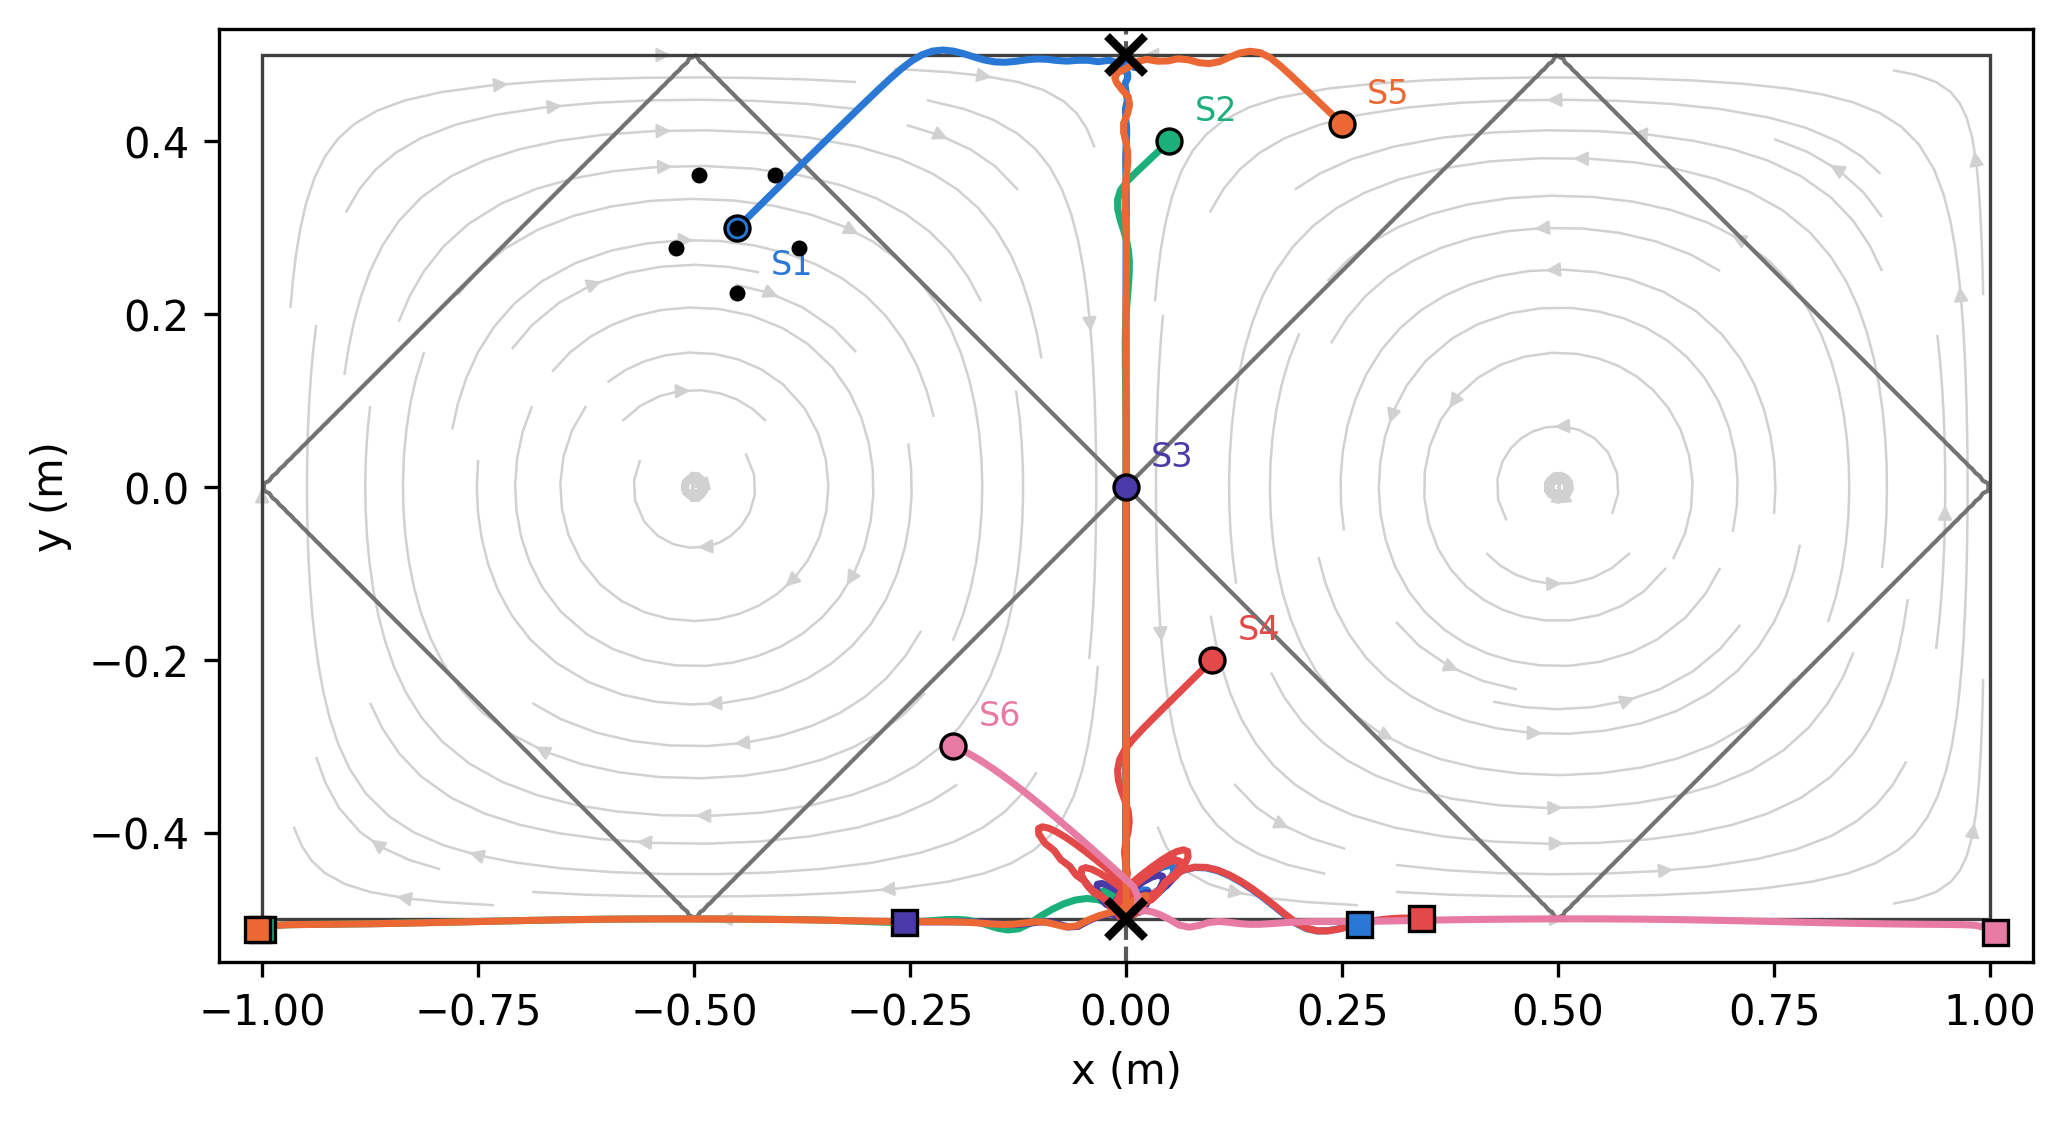
\includegraphics[width=0.34\textwidth]{figures/separatrix_trajectories.png}
    \caption{Noise-free $D$ tracker trajectories from six starts
    ($\bullet$), overlaid on the double-gyre streamlines and Okubo-Weiss
    diamonds. Every run reaches $x = 0$ and continues through the
    terminal saddle ($\times$) along the wall trench, ending at the
    square markers.}
    \label{fig:sep_trajectories}
\end{figure}

From the six starts of Fig.~\ref{fig:sep_trajectories}, all six reach the
separatrix and pass within 0.02 of the bottom saddle
$\mathbf{p}^*_1$ (closest approach 0.0003--0.0194 across runs). The six
starts lie between $0$ and $2.7\rho$ from the nearest trench segment
($\rho = 0.075$, the formation radius): two begin within one $\rho$ of
the structure, already satisfying (\ref{eq:flow_band}) at
initialization, and track it immediately; the other four start
$1.1\rho$ to $2.7\rho$ off it, none bracketing the separatrix, and
take 6, 13, 18, and 35 steps to reach it. Every run continues past
the terminal saddle rather than stopping there. This traces to the
floor $e$ on $\hat{\mathbf{H}}_D$ (Section~\mbox{III-D}):
near the well the estimated eigenvalues are indefinite and more than an
order of magnitude too small, so the capture test
$\lambda_1\lambda_2 \geq 0$ does not
fire even without noise.

\begin{table*}[!t]
\centering
\caption{Monte Carlo task success (\%): 10\,000 trials/cell from the
straddling start $(0, 0.35)$, random heading per trial, over the full
$\sigma_{uv} \times \sigma_p$ grid. (a) $D$ tracker and (b) $s_1$
tracker traverse success, both scored against the single far saddle
$\mathbf{p}^*_1$ a noise-free run from this start reaches. The $s_1$
transition falls entirely between $\sigma_{uv} = 0.001$ and $0.005$ at
every $\sigma_p$ shown, and at $\sigma_{uv} = 0$ entirely between
$\sigma_p = 0$ and $0.005$; both are resolved at 0.0005 spacing in
Fig.~\ref{fig:flip_resolution}. (c) $s_1$ tracker runs settling at
either saddle, the diagnostic that separates riding the separatrix in
the wrong direction from losing it: comparing (b) with (c) isolates the
tangent seed's contribution to failure.}
\label{tab:mc_success}
\footnotesize
\setlength{\tabcolsep}{4pt}
\begin{tabular}{r|rrrrr}
\multicolumn{6}{l}{(a) $D$ tracker: traverse success (\%)} \\
\hline
$\sigma_{uv}$ \textbackslash\ $\sigma_p$ & 0.000 & 0.005 & 0.010 & 0.020 & 0.050 \\
\hline
0.000 & 100.0 & 65.7 & 44.5 & 33.3 & 19.0 \\
0.001 &  99.6 & 63.2 & 45.6 & 32.9 & 19.1 \\
0.005 &  62.4 & 52.1 & 43.5 & 31.2 & 19.4 \\
0.010 &  43.7 & 40.7 & 37.0 & 28.8 & 18.7 \\
0.020 &  25.5 & 25.7 & 24.3 & 22.6 & 17.0 \\
0.050 &  16.0 & 16.2 & 15.8 & 16.1 & 14.9 \\
0.100 &  14.1 & 14.1 & 14.3 & 14.6 & 13.6 \\
0.200 &  13.5 & 12.4 & 12.8 & 12.8 & 12.4 \\
0.400 &  12.1 & 12.2 & 12.0 & 12.3 & 11.9 \\
0.800 &   4.8 &  5.4 &  5.1 &  5.4 &  5.2 \\
\hline
\end{tabular}
\hspace{1.5em}
\begin{tabular}{r|rrrrr}
\multicolumn{6}{l}{(b) $s_1$ tracker: traverse success (\%)} \\
\hline
$\sigma_{uv}$ \textbackslash\ $\sigma_p$ & 0.000 & 0.005 & 0.010 & 0.020 & 0.050 \\
\hline
0.000 & 100.0 &  1.3 &  0.0 &  0.0 &  0.0 \\
0.001 &  91.8 &  1.1 &  0.0 &  0.0 &  0.1 \\
0.005 &   0.0 &  0.0 &  0.0 &  0.0 &  0.0 \\
0.010 &   0.0 &  0.0 &  0.0 &  0.0 &  0.0 \\
0.020 &   0.0 &  0.0 &  0.0 &  0.0 &  0.1 \\
0.050 &   0.2 &  0.2 &  0.1 &  0.1 &  0.1 \\
0.100 &   0.5 &  0.4 &  0.4 &  0.4 &  0.3 \\
0.200 &   0.5 &  0.4 &  0.6 &  0.4 &  0.4 \\
0.400 &   0.5 &  0.5 &  0.5 &  0.6 &  0.5 \\
0.800 &   0.5 &  0.7 &  0.4 &  0.6 &  0.5 \\
\hline
\end{tabular}
\\[4pt]
\begin{tabular}{r|rrrrr}
\multicolumn{6}{l}{(c) $s_1$ tracker: settled at either saddle (\%)} \\
\hline
$\sigma_{uv}$ \textbackslash\ $\sigma_p$ & 0.000 & 0.005 & 0.010 & 0.020 & 0.050 \\
\hline
0.000 & 100.0 & 87.2 & 80.9 & 70.2 & 55.0 \\
0.001 &  99.7 & 87.0 & 81.0 & 70.4 & 55.1 \\
0.005 &  90.9 & 86.9 & 79.9 & 69.7 & 55.1 \\
0.010 &  79.8 & 78.0 & 74.7 & 68.1 & 55.5 \\
0.020 &  65.3 & 64.3 & 63.4 & 60.6 & 51.7 \\
0.050 &  46.8 & 47.1 & 47.1 & 46.7 & 46.3 \\
0.100 &  38.1 & 38.5 & 37.5 & 38.1 & 40.2 \\
0.200 &  37.1 & 36.8 & 38.2 & 37.9 & 38.4 \\
0.400 &  39.3 & 37.9 & 38.7 & 39.4 & 39.0 \\
0.800 &  40.2 & 40.4 & 39.3 & 40.1 & 40.0 \\
\hline
\end{tabular}
\end{table*}

Table~\ref{tab:mc_success}(a)'s traverse-success 50\% level, between
$\sigma_{uv} = 0.005$ and $0.01$ at $\sigma_p = 0$, coincides with the
open-loop $\nabla\hat{D}$ reliability threshold reported above: the
estimator, not the control law, sets the noise ceiling. Position noise
scales the same curve by $\|\mathbf{J}\|$, per (\ref{eq:sigma_eff})
($\sigma_p = 0.01$ alone and
$\sigma_{uv} = 0.01$ alone give nearly identical rates), and beyond the
cliff success does not fall to zero but levels off in the low tens of
percent through $\sigma_{uv} = 0.2$, the unbiased-random-walk floor
that only decays at the extreme extension $\sigma_{uv} = 0.8$.
Straddle retention, the failure metric of \cite{9}, decays cleanly with
no such floor (1.000 at zero noise, 0.589 at $\sigma_{uv} = 0.005$,
0.389 at 0.01). Tracking error (mean $|x_c|$) rises from 0.002 at
zero noise to 0.088 at the cliff and saturates near 0.27. Binning
the 40\,000 trials at $\sigma_{uv} \leq 0.01$, $\sigma_p = 0$ by
initial-heading quartile gives 75.9--77.1\% success per quartile,
confirming the isotropy of (\ref{eq:gain_ladder}).

Acquisition from off-structure starts was swept over the same noise
grid at $\sigma_p \in \{0, 0.01\}$, 1000 trials per cell, from two
clean-run starts $2.7\rho$ off the structure. The team reached the
trench network, closest approach under 0.05, in every one of the
20\,000 trials through $\sigma_{uv} = 0.02$ and in at least 97.5\% at
$\sigma_{uv} = 0.05$: acquisition itself is not the noise-limited
phase. Arrival at the one designated terminal saddle is a different
quantity, set by which branch of the network the descent reaches first;
from the start whose ride can reach either saddle, arrival holds near
40\% from zero noise through $\sigma_{uv} = 0.01$, one grid step later
than the straddling start's own cliff in Table~\ref{tab:mc_success}(a).
At zero noise this 40\% reflects outcome isotropy, not estimator
isotropy: the initial heading alone decides which branch the descent
reaches first, and heading is not uniform across the two outcomes it
produces here, while the estimator-error isotropy of (\ref{eq:gain_ladder})
holds and is confirmed above.

\subsection{Double Gyre: The $s_1$ Tracker}
\label{sec:results_oecs}

\subsubsection{Noise-free runs}
From the same six starts used for the $D$ tracker's own traverse
(Fig.~\ref{fig:sep_trajectories}), spanning both gyre halves, the
origin, and points off the structure entirely, the $s_1$ tracker reaches
the trench in 0 to 46 steps, longest from the farthest off-structure
start, and rides it through the eigenvector swap at the origin with no
dedicated crossing behavior: over the sweep of $r_{\text{band}}$ from
0.05 to 0, the degenerate-frame
guard never fires once, so the
crossing is carried entirely by ordinary tangent selection
(\ref{eq:tangent_select}). All six runs settle at a saddle, within
0.011 to 0.022 of it, at whichever one their initial tangent
orientation resolves toward: four at $\mathbf{p}^*_1 = (0, -0.5)$ and
two at $\mathbf{p}^*_2 = (0, 0.5)$. The mean
path gap against the $D$ tracker's own trajectory from the same start,
measured over the common on-trench portion of each run, is 0.020 to
0.322 across the six. The gap is largest where the two trackers commit
to different saddles. That happens from a start equidistant enough that
the seeded tangent and the $D$ tracker's own flow-tested tangential term
do not agree; where they commit to the same saddle the two paths are visually
coincident until the $s_1$ tracker settles and the $D$ tracker continues
onto the crossing wall trench, the divergence the floor $e$ of
Section~\mbox{III-D} already predicts for the $D$ tracker's own command. This is the
designed contrast with Fig.~\ref{fig:sep_trajectories}: both trackers
traverse the same network from the same objective starting condition,
but only the $s_1$ tracker's terminal test is built to fire reliably at
what it finds.

\begin{figure}[!t]
    \centering
    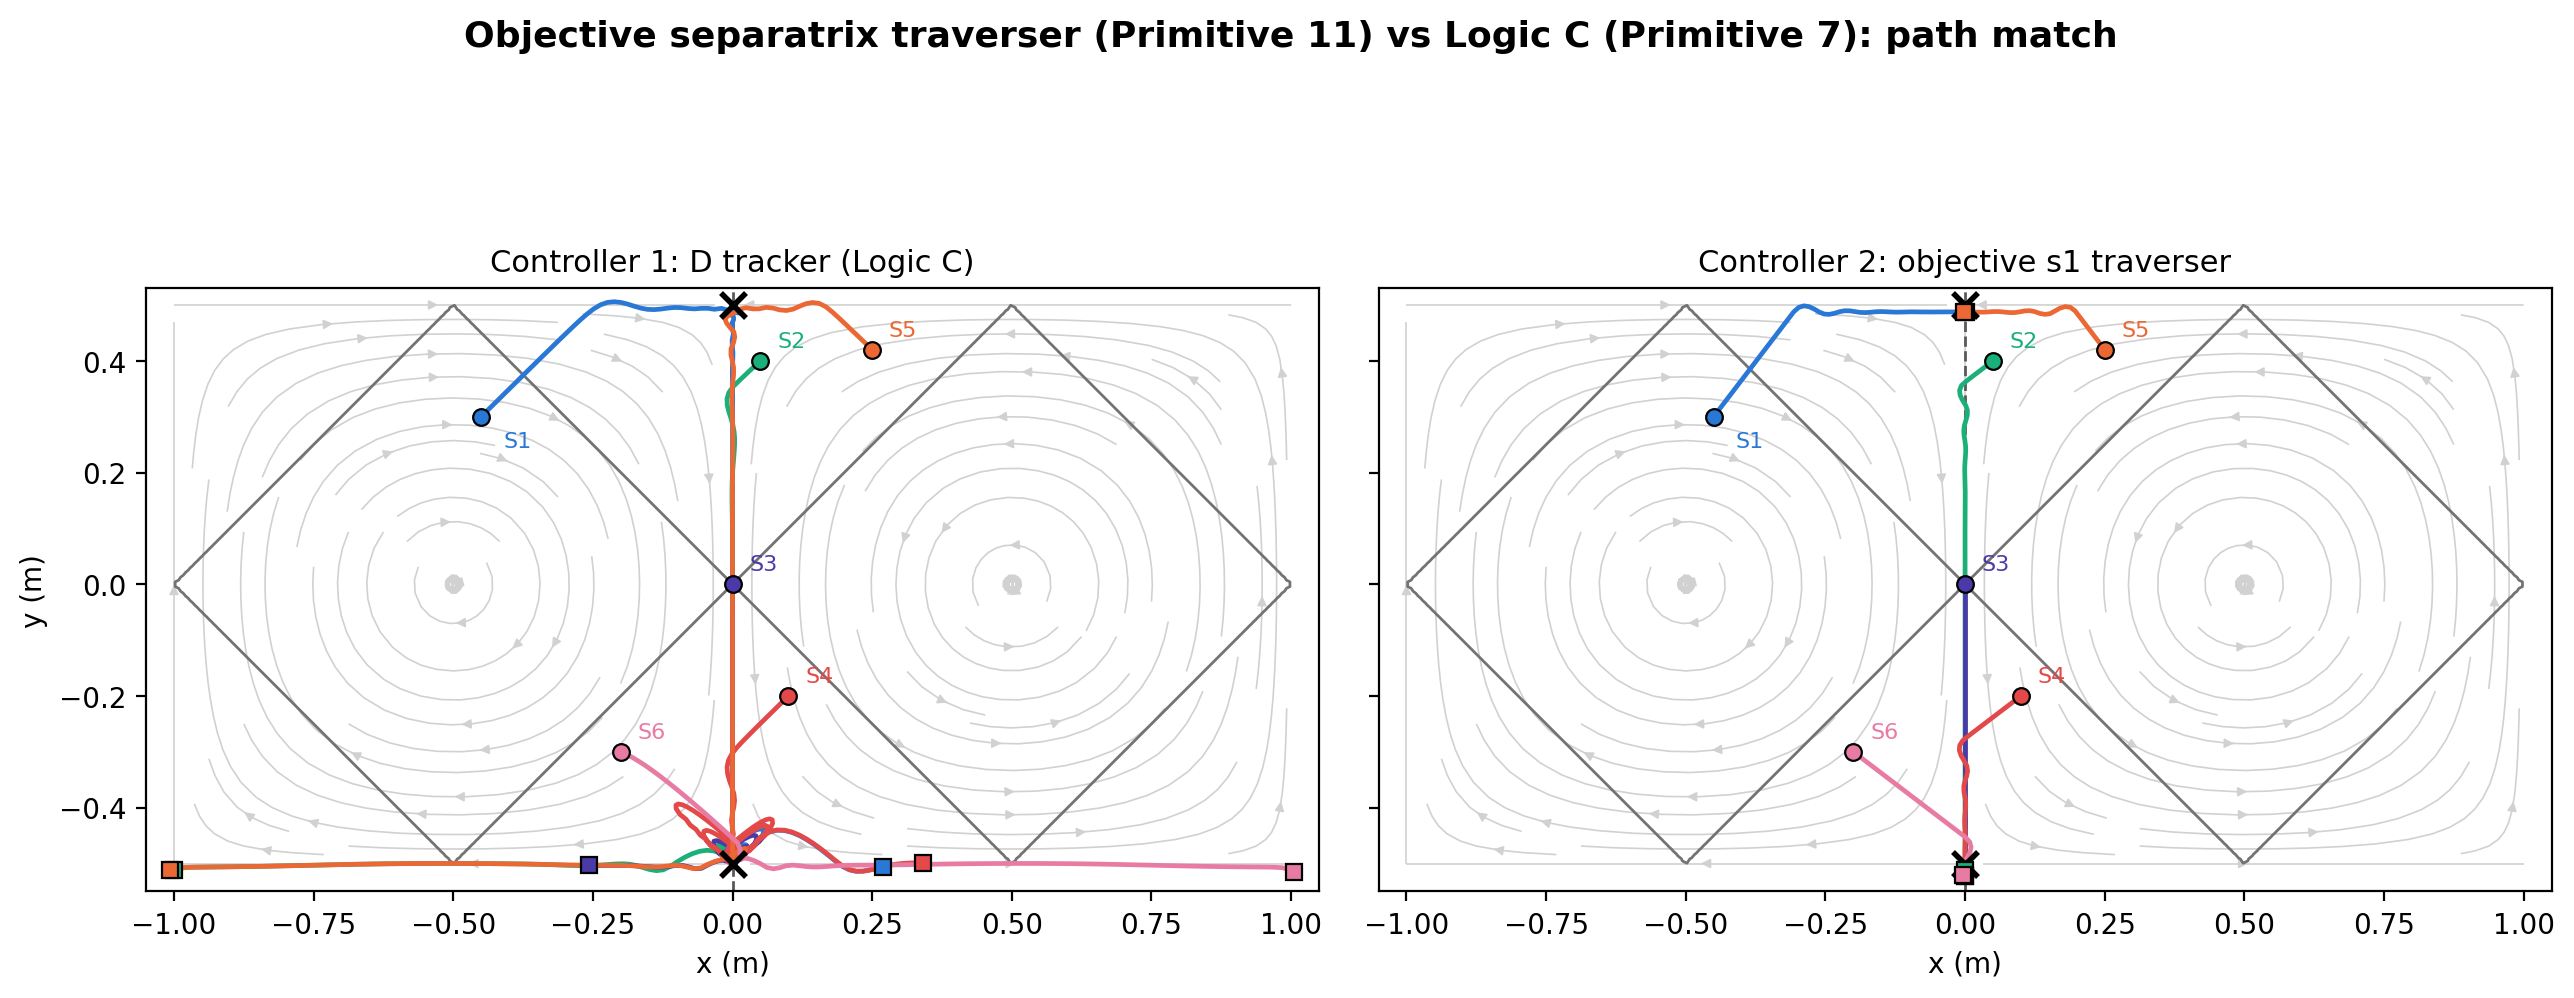
\includegraphics[width=0.34\textwidth]{figures/traverse_vs_logic_c.png}
    \caption{$s_1$ tracker versus $D$ tracker, six matched starts,
    noise-free. Both traverse the same network through the eigenvector
    swap at the origin; the $s_1$ tracker captures at the saddle its
    tangent orientation resolves toward, while the $D$ tracker
    continues onto the crossing wall trench past every saddle it
    reaches.}
    \label{fig:traverse_vs_logic_c}
\end{figure}

\subsubsection{Objectivity}
The objectivity demonstration follows the rotating-frame protocol of
Section~\mbox{V-D}. Fig.~\ref{fig:oecs_objectivity} shows the
outcome. The $s_1$ tracker's two runs are the same material path: final
gap 0.025, mean gap 0.014 over the common steps, with mean distance to
the true trench network of 0.000 (inertial) and 0.005 (rotating); both
runs traverse the same eigenvector swap and capture at the same bottom
saddle. The $D$ tracker's two runs are not: the rotating observer's $D'$
landscape (\ref{eq:D_not_objective}) and swirl-contaminated flow
measurement carry the team off the separatrix entirely, to a mean
trench-network distance of 0.052 (ten times its inertial value of
0.005) and a final gap of 1.219 from its inertial twin, ending in the
gyre interior where no structure exists. Under a rotating observer the
$D$ tracker follows a frame artifact; the $\mathbf{S}$-based tracker
does not, past the single seeding instant
Proposition~\ref{prop:equivariance} identifies, which confines the
frame dependence to that one instant rather than carrying it for the
life of the run.

\begin{figure}[!t]
    \centering
    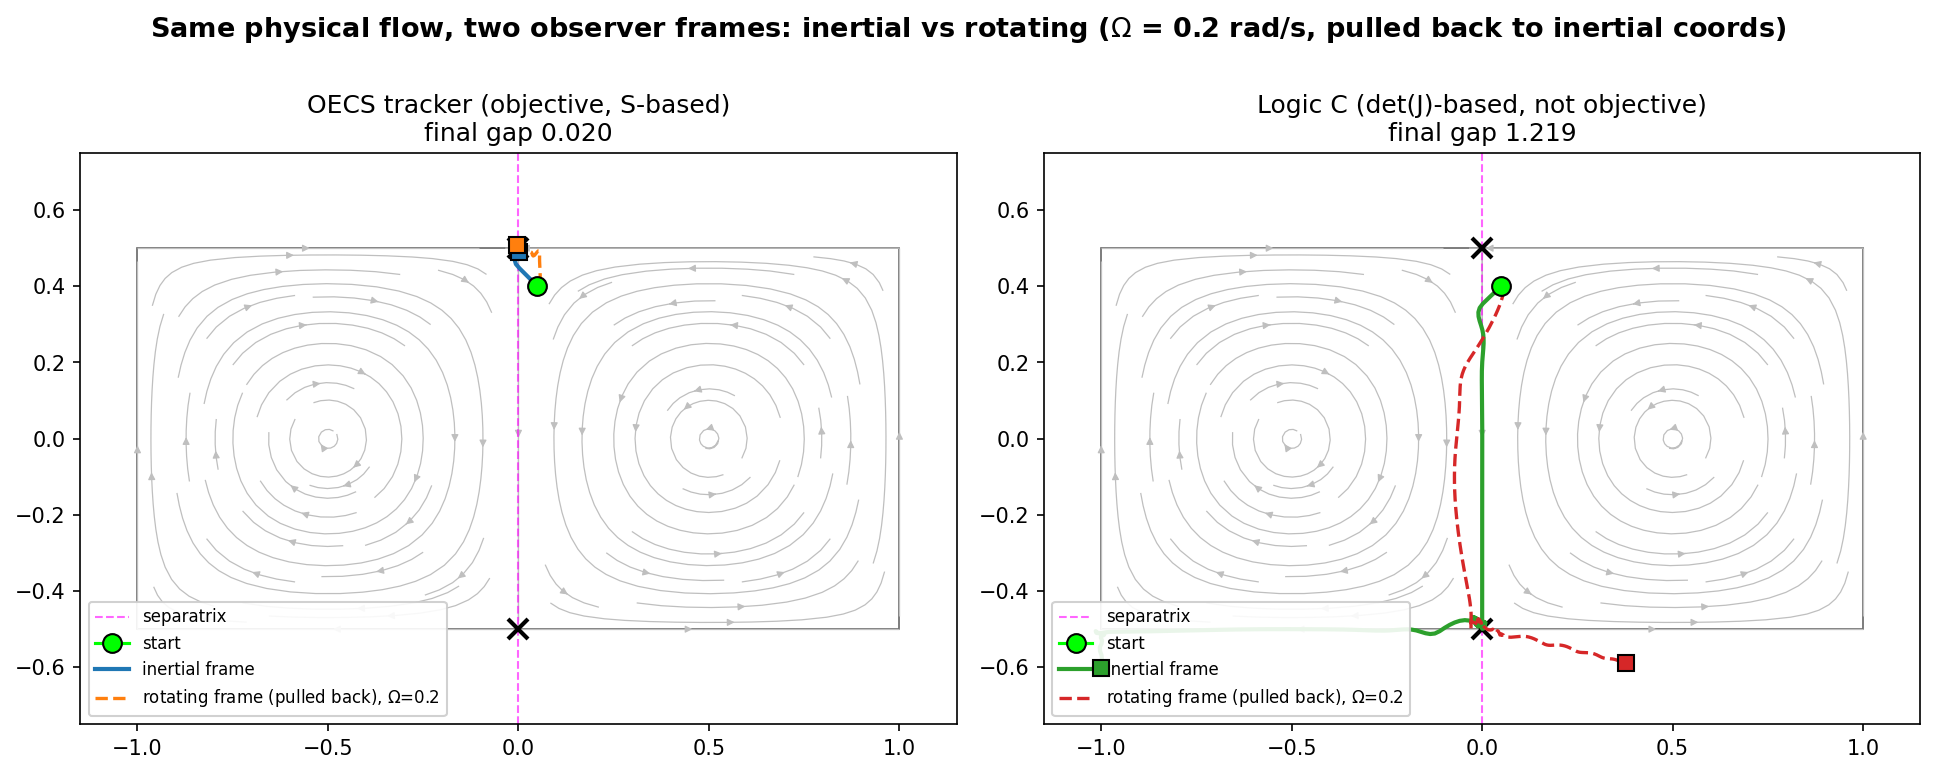
\includegraphics[width=0.38\textwidth]{figures/oecs_objectivity.png}
    \caption{Objectivity experiment: each controller run in the
    inertial frame (solid) and in a frame rotating at $\Omega = 0.2$
    rad/s (dashed, pulled back to inertial coordinates). Left: the
    $s_1$ tracker's trajectories coincide (final gap 0.025). Right: the
    $D$ tracker's rotating-frame run leaves the separatrix (final gap
    1.219), the artifact predicted by (\ref{eq:D_not_objective}).}
    \label{fig:oecs_objectivity}
\end{figure}

\subsubsection{Noise robustness}
Table~\ref{tab:mc_success}(b) reports traverse success for the $s_1$
tracker over the same noise grid, scored against $\mathbf{p}^*_1$. The
zero-noise tracking error is 0.0075, about five times the $D$ tracker's
0.0016. The ultimate bound (\ref{eq:iss_bound}) predicts the opposite
ranking, since $a_{\perp,s_1} > a_{\perp,D}$ at this operating point;
the ordering instead matches the discrete stability condition of
Table~\ref{tab:bandwidth}, which the $s_1$ tracker crosses over the
outer half of the structure.
Under noise the two trackers do not degrade the same way, and the
difference is not one of degree. (The widened $0.60$ exit box recovers
30 of the 54 trials that the $D$ tracker's own $0.52$ box would have
scored as domain exits at $\sigma_p = 0.005$, all of which exit at $y
\in [0.520, 0.529]$, a hair past the tighter box, while still
converging.) Fig.~\ref{fig:flip_resolution}(a)
resolves the transition at 0.0005 spacing: success falls from 91.8\% at
$\sigma_{uv} = 0.001$ through 43.5\% at 0.002 to 6.7\% at 0.003, and by
$\sigma_{uv} = 0.005$ it is 0.0\%, a floor it holds out to 0.008. The
$D$ tracker's corresponding column falls only from 62.4\% to 43.7\%
across the same $\sigma_{uv} = 0.005$--$0.01$ span.

What separates them is visible only by comparing
Table~\ref{tab:mc_success}(b) with panel (c). Where far-saddle success
is 0.0\% at $\sigma_{uv} = 0.005$, 90.9\% of those same runs still
settle cleanly at a saddle. The team has not lost the structure, become
erratic, or collapsed: it rides the separatrix competently and settles,
in the wrong direction. The fraction of runs whose ride commits toward
$\mathbf{p}^*_1$ is 100.0\% at zero noise, 91.9\% at
$\sigma_{uv} = 0.001$, and 0.1\% at 0.005. This is a sign inversion,
not a decay toward chance, and it is what makes the far-saddle column
the honest score: a near-saddle settle is a directional failure of the
ride, indistinguishable in every other recorded quantity from a
success.

The mechanism is the one-time flow read that seeds
$\mathbf{t}_{\text{ref}}$
on the first tracking step. At this start the differential flow signal
across the six sample points is small (span $\approx 0.12$), comparable
to $\sigma_{uv}$ in the 0.001--0.003 range, so the sign it resolves is
decided by noise well before the transverse channel's own tolerance is
approached. Against peak flow, $\pi A \approx 0.314$, $\sigma_{uv} =
0.002$ is a modest 0.6\%; against this 0.12 differential span, the
denominator the tangent decision actually consumes, the same noise is
1.7\%, which is the reading that explains the seed's fragility. Because
the decision is made once and then carried forward by continuity, a
perturbation large enough to flip it does not merely degrade the run, it
commits the whole ride to the opposite branch. The noise is comparable
to that 1.7\%-scale signal, so above the threshold nearly every draw
crosses it in the same direction rather than half reversing and half
not: the flip is near-total, not an even split.

Table~\ref{tab:mc_success}(b) shows the same collapse along the
$\sigma_p$ axis at $\sigma_{uv} = 0$ (100.0\% at $\sigma_p = 0$, 1.3\%
already by $\sigma_p = 0.005$) with no points between to show its
shape; Fig.~\ref{fig:flip_resolution}(b) resolves it at the same
0.0005 spacing, 10\,000 trials/cell. Success falls from 99.8\% at
$\sigma_p = 0.0005$ through 63.6\% at 0.002 to 6.6\% at 0.004,
crossing 50\% between $\sigma_p = 0.002$ and 0.0025, close to panel
(a)'s own $\sigma_{uv}$ crossing. Position noise enters through the
same effective-measurement-error coupling
$\mathbf{J}(\mathbf{p}_i)\boldsymbol{\xi}_i$ of (\ref{eq:pos_noise}),
so at this test point, where the $D$ tracker's own noise grid gave
$\|\mathbf{J}\| \approx 1$, a given $\sigma_p$ degrades the seed by
roughly the same amount as an equal $\sigma_{uv}$ would. The two panels
are one finding measured on two axes, not two failure modes: whichever
noise channel is active, it is the one-time flow read that fails first,
well before the transverse channel's own regulation would predict
trouble.

Straddle retention, conditioned on the same $\mathbf{p}^*_1$ contact
(a trial that stops at the wrong saddle has no straddle-to-$\mathbf{p}^*_1$
history to report), stays below success at every level shown
(73.2\% against 91.8\% at $\sigma_{uv} = 0.001$, 47.6\% against 71.5\%
at 0.0015, reaching zero by 0.004 where success itself is already under
1\%), consistent with straddle being the stricter condition once both
are scored against the same target. The $D$ tracker's own straddle
retention decays more gradually over the same interval (0.589 at 0.005,
0.389 at 0.01) and does not depend on which saddle is reached, since its
target never moves.

The tangent-selection mechanism itself
(\ref{eq:tangent_select}) is not the source of this fragility: it uses
only the already-computed gradient projections, and the tangent
direction
survives noise past the point every gradient-based quantity approaches
chance, which still applies to whichever eigenvector it currently
selects. The
fragility is specific to the sign convention at the seed, a single
comparison against the ambient flow.

\begin{figure*}[!t]
    \centering
    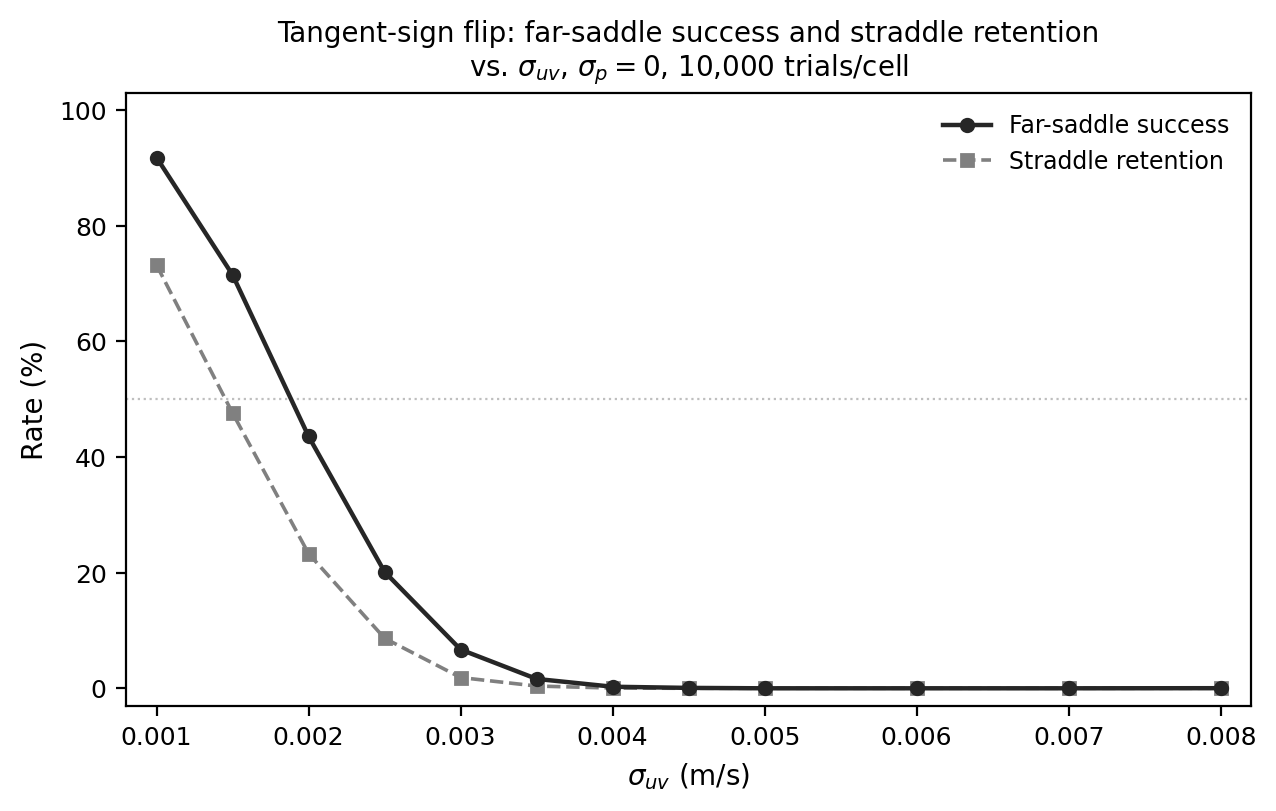
\includegraphics[width=0.78\textwidth]{figures/flip_resolution.png}
    \caption{Resolving the tangent-sign flip: far-saddle success and
    straddle retention (both conditioned on reaching $\mathbf{p}^*_1$),
    10\,000 trials/cell, at 0.0005 spacing on each axis. (a) Against
    $\sigma_{uv}$, $\sigma_p = 0$: success crosses 50\% between
    $\sigma_{uv} = 0.0015$ and 0.002 and reaches a sub-1\% floor by
    0.005, held out to 0.008. (b) Against $\sigma_p$, $\sigma_{uv} = 0$:
    the same decline, crossing 50\% between $\sigma_p = 0.002$ and
    0.0025. The transition is resolved and continuous on both axes; what
    is abrupt is the outcome it selects between, since runs on either
    side of it settle at a saddle with comparable reliability
    (Table~\ref{tab:mc_success}(c)) and differ in which one.}
    \label{fig:flip_resolution}
\end{figure*}

Open-loop checks at the nominal radius confirm the structural picture
behind these margins. The fitted shear strain at three test points is
at the $10^{-4}$ level (analytic value zero); the fitted
$\hat{\mathbf{H}}_{s_1}$ eigenvalues are $[-0.011, 0.000]$ and smaller,
negative semidefinite as Remark~\ref{rem:s1hess} requires; the
transverse component of (\ref{eq:grad_s1}), evaluated at $(0.03, 0.25)$,
recovers the restoring slope $4.0$ per unit offset against the analytic
transverse curvature $6.9$ at that point, the two values entering
Table~\ref{tab:bandwidth}; and at $\sigma_{uv} =
0.01$ the median direction
error of $\mathbf{e}_2$ is $4.5^\circ$, against $44^\circ$ for
$\nabla\hat{s}_1$ and $41^\circ$ for the $\hat{\mathbf{H}}_D$
eigenvector ($2\times 10^4$ draws per level).

\subsection{Ocean HFR: Both Trackers from a Shared Start}
\label{sec:results_ocean}

The $D$ tracker and the $s_1$ tracker were each run from a single
shared start north of the channel entrance,
$(34.41^{\circ}\mathrm{N}, -120.39^{\circ}\mathrm{W})$, at the
operating point of Table~\ref{tab:params}. Over the 28~h trial both
controllers descend through the channel entrance and track the same
ridge through the bifurcation, their paths overlapping for nearly the
entire record; they separate only in the final stretch, where the $D$
tracker continues to landfall on the middle island's north coast while
the $s_1$ tracker is still closing on the same target when the 28-h
budget ends.
Fig.~\ref{fig:ocean_ftle}
places both trials against the 24-h forward-time FTLE field, computed
offline over the same window in the style of \cite{17}; both paths
follow the dominant FTLE ridge running from the channel entrance to the
bifurcation closely, without the ridge being available to either
controller at any point, only the local estimates built from the
current samples at the formation ($\hat{D}$ and $\hat{\mathbf{g}}$ for
the $D$ tracker, $\hat{s}_1$ and its eigenframe for the $s_1$ tracker).

\begin{figure}[!t]
    \centering
    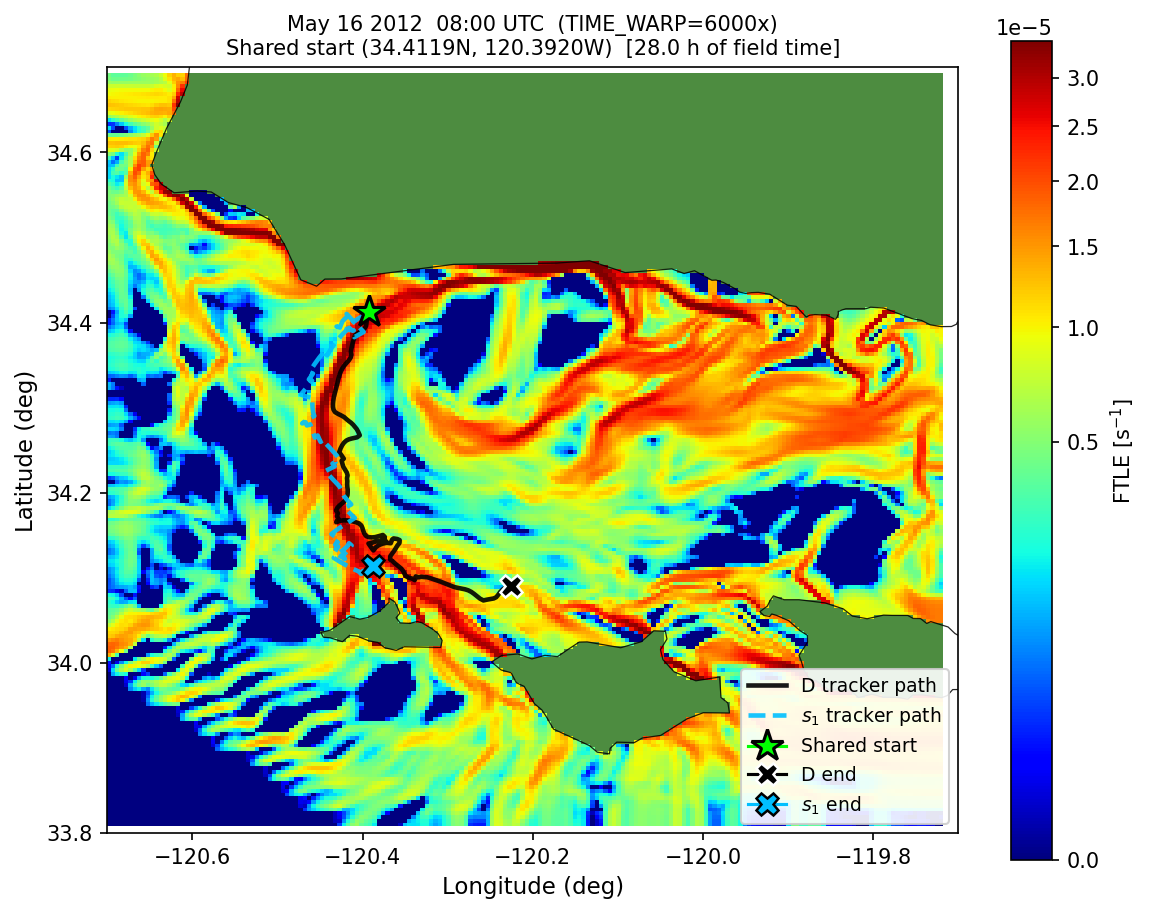
\includegraphics[width=0.38\textwidth]{figures/ocean_ftle_trajectory_overlay_2km.png}
    \caption{28-h $D$ and $s_1$ tracker paths, from a single shared
    start, over the 24-h forward FTLE field computed offline from the
    same 2~km data. Both paths follow the dominant ridge from the
    channel entrance to the bifurcation and separate only near
    landfall, where the $D$ tracker reaches the middle island's north
    coast and the $s_1$ tracker is still converging on the same target
    when the 28-h record ends.}
    \label{fig:ocean_ftle}
\end{figure}

Forward FTLE recomputed at four anchor times across the record (0, 5,
10, and 16~h, each integrated 12~h forward) confirms that the dominant
ridge persists while the finer structure downstream evolves: the
experiment is genuinely time-varying, and each controller sees only the
instantaneous samples at its own formation position.

A $10 \times 10$ grid of starts jittered $\pm 0.05^{\circ}$ around the
validated $D$-tracker start shows the outcome is not knife-edge
sensitive to the initial condition: 84 of the 100 land on the same
middle-island branch as the validated trial, with the rest carried onto
a western branch by starts nearest the jitter-box edge furthest from
the ridge.

The $s_1$ tracker relies on the terminal test (\ref{eq:capture_test})
alone; a genuine two-dimensional minimum of $s_1$ is not reached within
the 28-h budget from this start, so the tracker's mean $\hat{s}_1$
along the ride is the tracked value rather than a certified settle.
This is an outcome of the same law, not a failure of it: absent a
stationary point of $s_1$ close enough to the ride to satisfy
(\ref{eq:capture_test}), the $s_1$ tracker behaves as a traverser,
reading the same ridge structure the $D$ tracker does from the
objective strain term alone. Ground truth on this field, computed
offline from the full radar grid in the style of \cite{17,36} (TRAP
cores as local minima of $s_1$ at each hourly frame), is generic,
unlike the double gyre: isolated degeneracies and cores that move
between frames, so this experiment also exercises tangent selection
(\ref{eq:tangent_select}) on a live field where neither the eigenframe
nor the trench network is axis-aligned. The method runs unmodified on
measured data for 28~h and produces a path that follows the dominant
FTLE ridge, the same demonstration the $D$ tracker gives from the same
start.

\section{Discussion}
\label{sec:discussion}

Instantaneous criteria of this
kind are not in general reliable indicators of the material transport
skeleton \cite{16}; the double gyre used throughout is a favorable
special case in which the $D$ trench coincides exactly with the
separatrix, and the ocean agreement is an empirical finding on that one
record, not a guarantee that carries to arbitrary flows.

Every quantity in (\ref{eq:oecs_law}) transforms equivariantly under a
time-dependent rotation of the observer
(Proposition~\ref{prop:equivariance}). The scalars $\hat{s}_1$ and $r$
are invariant, the gradient and the eigenframe co-rotate, the projector
is built from a co-rotating unit vector, and the saturation preserves
direction. The commanded velocity therefore co-rotates, and the
closed-loop trajectory is the same material path in any frame. One
exception is confined to a single instant: on the first tracking step,
the sign reference falls back to the measured flow. Every step
thereafter carries orientation forward by continuity, which is
covariant. A rule that instead resolved (\ref{eq:tangent_select}) by
alignment with the flow at each step would inherit the observer
dependence at every step rather than once.

\subsection{Implications}
\label{sec:prior_comparison}

Tracking a trench is structurally harder than tracking a regular level
set: a level set is fixed by first-order information, while the trench
lives exactly where that gradient vanishes in the normal direction, so
controller and proof alike must synthesize the missing direction from
curvature, the price paid in the eigenstructure dependence, mode
switching, and tube assumptions of the stability analysis. A
controlled head-to-head against the straddle family \cite{9,10,11} and
the onboard-FTLE strategy of \cite{13} on identical fields, formations,
and noise is future work; Table~\ref{tab:assumptions} compares the
stated assumptions instead, each cell sourced from the cited papers'
own text.

\begin{table}[!t]
\centering
\caption{Stated assumptions, this paper against the nearest prior
robotic structure-tracking methods.}
\label{tab:assumptions}
\scriptsize
\setlength{\tabcolsep}{3pt}
\begin{tabular}{@{}l>{\raggedright\arraybackslash}p{0.19\linewidth}>{\raggedright\arraybackslash}p{0.19\linewidth}>{\raggedright\arraybackslash}p{0.19\linewidth}@{}}
\hline
& \textbf{This paper} & \textbf{\cite{9,10,11}} & \textbf{\cite{13}} \\
\hline
Init. & any six-robot config., on or off structure & straddling formation already on the manifold, opposite sides & center robot already on the boundary $B_u$ \\
Structure ID & not required in advance & assumed known (which boundary is straddled) & not required; located from the FTLE field itself \\
Sensing & one synchronous velocity sample per robot, no history & continuous velocity measurement per robot & a sensing grid advected over a finite window \\
Advection & robots not advected; field is sampled, not physically sat in & robots advected by the flow (their eq.~1a) & sensing grid particles advected by construction \\
Estimated & full local quadratic model: gradient and curvature of $D$ and $s_1$ & boundary crossing only, via a PIM triple & FTLE ridge location, via finite-time integration \\
Terminal behavior & traverses (both) or certifies a terminal core ($s_1$) & maintains the straddle; no terminal state & re-locates the ridge each window; no terminal state \\
\hline
\end{tabular}
\end{table}

Two grounds keep the comparison structural rather than empirical.
First, initialization is not a detail of these methods but the premise
of their guarantees: \cite{9}'s straddling formation control is stated
for robots already on opposite sides of the boundary, and \cite{13}
assumes the center robot starts on $B_u$. Running either from an
off-structure start is outside its own stated problem, and running this
paper's method from a pre-straddled start discards the acquisition
result of Fig.~\ref{fig:basin_map}. Second, the two plants differ:
\cite{9,10,11,12} and \cite{13} both write the robot's velocity as the
commanded term plus the ambient flow (their eq.~1a in \cite{9}; eq.~5a
in \cite{13}), so their robots are advected, while this paper's are
not (Section~\ref{sec:problem_statement}). One simulator cannot host
both without altering one of them.

The nearest prior work reports its own limitation at exactly the
structure this paper is built around: robots following \cite{9}'s
strategy ``tend to veer away from the tracked LCS as they approach a
local saddle/hyperbolic point in the flow,'' because ``the flow
reverses direction on the other side of the saddle point'' in both
their flow-tank and ocean trials. The $D$ tracker traverses through
that same crossing, and the $s_1$ tracker settles at it.


\subsection{Objectivity Tradeoffs}
\label{sec:objectivity_tradeoff}

Table~\ref{tab:budget} places both surrogates on the same noise rung, so
the choice between them is not one of accuracy. It is which channels
carry constants. Everything derived from $\hat{D}$ carries the observer
term $O(\mathrm{Ro})$, and $\hat{\mathbf{H}}_D$ carries the
unmodelled-derivative floor $e$ as well; $\hat{s}_1$ carries neither and
is exposed instead at $1/r$, which belongs to the strain field rather
than to the sensing. The rotating-frame gaps, 0.025 against 1.219, are
the first of those constants made visible: it contains no $\nu$, no
$\tilde{\rho}$, and no formation geometry, so no estimator improvement
removes it.

The double gyre is a favorable case for that comparison and a
misleading one for its cost. Objectivity buys no extra reach there,
since the two trenches coincide exactly, and the identically vanishing
shear keeps $r$ away from zero, so the $1/r$ exposure the generic ocean
field loads is barely tested. What the double gyre does expose is
rate. The $D$ tracker
normalizes by a curvature and holds $a_\perp = 1$ along the whole
structure; the $s_1$ tracker takes $a_\perp = g_\perp\kappa_\perp$ from
the field, and at the operating point of Table~\ref{tab:params} that
puts the outer half of the structure past the discrete stability
threshold (Table~\ref{tab:bandwidth}). Both consume the same fit, so the
choice is one function call rather than a new estimator or formation.

\subsection{Failure Modes}
\label{sec:failure_modes}

Three behaviors fall outside Section~\mbox{IV-D}. The fit is
ill-conditioned whenever the six sampling points drift toward a common
conic (Proposition~\ref{prop:conic}); monitoring
$\kappa(\boldsymbol{\Phi})$ and adding a shape-maintenance term is the
direct mitigation, not implemented here. Noise can chatter the $D$
tracker across
the band boundary (\ref{eq:flow_band}), which costs only along-trench
speed since both branches of (\ref{eq:tau}) share the transverse
dynamics (\ref{eq:n_dynamics}). And the strain eigenframe is fragile
where $\mathbf{S}$ approaches isotropy, the $1/r$ column of
Table~\ref{tab:budget}. Tangent selection (\ref{eq:tangent_select}) is
the defense once the ride is underway, comparing gradient alignment
rather than eigenvector identity; the residual risk of a wrong branch at
a crossing under heavy noise is damped but not excluded by the latch on
(\ref{eq:capture_test}), and the generic ocean field exercises the whole
mechanism.

\subsection{Limitations}
\label{sec:limitations}

The $s_1$ tracker's tangent sign, resolved once from the ambient flow
at the first tracking step, is only
as reliable as the local differential flow signal is large relative to
the noise level; at the straddling start of Table~\ref{tab:mc_success}(b)
that signal is weak enough that the resolved sign passes through an even
split near $\sigma_{uv} = 0.002$ and inverts almost completely by
$0.005$ (Fig.~\ref{fig:flip_resolution}). Three
unimplemented alternatives trade this differently: a start-independent
convention (e.g., a fixed world-axis component of $\mathbf{e}_2$)
removes the flow dependence at the cost of an arbitrary discontinuity,
the same kind the degenerate-frame guard's own flow-only fallback
already accepts; a
confidence check on the seed converts a wrong commitment into a longer
settling phase at the cost of a noise-level estimate the controller does
not otherwise need; and re-fitting the sign over several early steps
trades the single-instant risk for a short transient of ordinary
tracking-error exposure, closer in spirit to how time-to-band already
absorbs acquisition. None was implemented, since the finding was made
late enough in the noise-sweep validation that a design change here
would need its own noise sweep to verify. That is future work, alongside
the hardware validation above.

All results are from simulation; hardware validation on the Decabot
testbed is planned as a follow-on study. Throughout, robot motion is
commanded by the control law, not advected by the sampled flow
(Section~\ref{sec:problem_statement}). For the Decabot testbed this is
exact rather than approximate: the robots are not immersed in anything,
and the field is encoded and read rather than physically experienced
\cite{33}. On the ocean field it is an extrapolation: the commanded
speed cap is far above realized ocean currents at this operating point,
but the assumption itself is untested against real advection and is a
scope boundary for that experiment, not a validated one. The double-gyre noise sweeps
use the static field ($\varepsilon = 0$). A spot check at
$\varepsilon = 0.1$, $\omega_{dg} = 2\pi/10$ runs the $D$ tracker down
the oscillating trench at zero noise: the instantaneous trench swings
$\pm 0.116$ in $x$ with peak speed equal to 62\% of the commanded
speed cap, and the tracker holds it with mean transverse offset 0.006
and maximum 0.015, with no time-derivative term in the controller. The
ocean experiments show the same behavior on a measured field; no
analytic guarantee is offered for either case.


No start settles at a gyre core: descent of $\hat{D}$ from the
rotation-dominated interiors reaches the trench network within the
500-step horizon in all 20\,000 runs, so the basin boundary is not the
Okubo-Weiss partition. The map is instead the watershed of the descent
composited with the flow direction on the acquired branch: a central
diamond of direct traverses (26.9\%), an upper region that rides the
top wall to $\mathbf{p}^*_2$ and continues to $\mathbf{p}^*_1$
(20.5\%), interleaved with north-branch losses at the $\mathbf{p}^*_2$
junction (5.6\%), and lower and outer watersheds whose boundary-trench
rides leave the domain without reaching $\mathbf{p}^*_1$
($47.1\%_{\text{grid loss}}$), since the walls are also valley lines
of $D$ and the bottom wall carries flow away from $\mathbf{p}^*_1$. The
grid's own success rate, direct plus top-wall arrivals, is
$26.9\% + 20.5\% = 47.4\%$, agreeing within sampling noise with a
separate $47.1\%_{\text{random}}$ from $n = 10{,}000$ uniformly random
starts and headings; the near-match of that
$47.1\%_{\text{random}}$ to the unrelated grid-loss figure
$47.1\%_{\text{grid loss}}$ above is a coincidence of digits between two
different quantities, not a second confirmation. Prior
adaptive-navigation primitives
\cite{27}, \cite{28} report local convergence without basin estimates.

\section{Conclusion and Future Work}
\label{sec:conclusion}
\label{sec:future}

This paper presented one cooperative estimator and two trackers built
on it. A six-robot formation, proved minimal for the unconstrained
quadratic model, recovers the local
quadratic model of a planar flow from a single synchronous sample, and
with it both terms of the splitting identity $D = \omega^2/4 - s_1^2$,
with closed-form, heading-isotropic noise gains verified to $0.3\%$.
The $D$ tracker solves Problem 1, riding the connected trench network of
$D$ on a modified Newton step, with a Lyapunov certificate and a
network-traversal theorem. The $s_1$
tracker solves Problem 2, riding the same network from the strain term
alone, with a terminal test built only from the objective gradient,
because $s_1$'s minimum is recoverable from a first derivative of the
fit where $D$'s needs a Hessian sign the estimator delivers correctly
in magnitude but not reliably in sign (Remark~\ref{rem:s1hess},
Table~\ref{tab:budget}); its frame
equivariance was demonstrated in closed loop rather than asserted: the
same material curve in either observer frame (gap 0.025), where the $D$
tracker follows a frame artifact (gap 1.219). Monte Carlo sweeps placed
the $D$ tracker's failure cliff exactly at the estimator's
gradient-reliability threshold, so the estimator, not the control law,
sets its noise ceiling; the $s_1$ tracker's own noise ceiling is set
one level earlier by a different mechanism, the reliability of the
one-time flow-seeded tangent sign rather than the estimator's gradient
accuracy. On
real Santa Barbara Channel currents the $D$ tracker followed a coherent
ridge for 28 hours to a consistent landfall reproduced by 84 of 100
nearby starts, and the $s_1$ tracker, started on that same ridge, rode
the same network structure for 28 hours from the objective strain term
alone. Every capability rests on the same premise: a team that can
sense second-order structure locally does not need a precomputed FTLE
field.

Five extensions are direct. A time-derivative correction term,
analyzed against the analytic $\varepsilon > 0$ double gyre, would
extend the stability results to time-varying fields with a quantified
bound. Online formation reshaping would protect the conditioning of
$\boldsymbol{\Phi}$, and a step-halving sweep would separate the $s_1$
tracker's discretization limit cycle from its estimation error
(Table~\ref{tab:bandwidth}). Hardware deployment on the Decabot testbed would
close the loop on physical robots and test the no-advection assumption
directly. Extension to three dimensions raises the estimation stakes:
ten coefficients per component, so ten robots, or a reduced-order
estimator. And targets other than critical points, transient attracting
profiles, eddy cores, and other non-critical-point structures, are a
natural next object for the same estimator and a separate paper.

\appendices

\section{Proofs}
\label{app:proofs}

\begin{IEEEproof}[Derivation of the noise ladder (\ref{eq:gain_ladder})]
Place the ring robots at $\mathbf{p}_j = \rho(\cos\theta_j,
\sin\theta_j)$ with $\theta_j = \psi + 2\pi j/5$, $j = 0, \ldots, 4$, and
the sixth robot at the centroid, leaving the ring phase $\psi$ free.
Every entry of $\boldsymbol{\Phi}^\top\boldsymbol{\Phi}$ is a ring sum of
a monomial in $\cos\theta_j, \sin\theta_j$ of degree at most four, hence a
combination of the fifth roots of unity; every such sum vanishes unless
its index is a multiple of five, so only the phase-independent $n = 0$
term survives at every order through the fourth. The odd sums vanish
identically and the surviving even sums are constants,
$\sum_j\cos^2\theta_j = \sum_j\sin^2\theta_j = \tfrac{5}{2}$,
$\sum_j\cos^4\theta_j = \tfrac{15}{8}$, and $\sum_j\cos^2\theta_j
\sin^2\theta_j = \tfrac{5}{8}$, independent of $\psi$.

The gains follow. Every basis function of (\ref{eq:basis}) except the
constant vanishes at the origin, so the center robot's reading fixes
$\hat{a}_1$ and $\sigma_{a_1} = \sigma_{uv}$. The vanishing odd sums
leave the linear block orthogonal to the constant and quadratic blocks,
so the system separates; the linear block inverts against
$\tfrac{5}{2}\rho^2$ and the quadratic block against the fourth-order
sums scaled by $\rho^4$. Row norms of $\boldsymbol{\Phi}^{-1}$ then give
(\ref{eq:gain_ladder}). No power sum depends on
$\psi$, so neither do the gains. The gradient rows are orthogonal with
equal norm, making the gradient block of $\sigma_{uv}^2
\boldsymbol{\Phi}^{-1}\boldsymbol{\Phi}^{-\top}$ exactly
$\tfrac{4}{10}\sigma_{uv}^2\rho^{-2}\mathbf{I}$, isotropic for every
heading.
\end{IEEEproof}

\begin{IEEEproof}[Proof of Theorem~\ref{thm:separatrix}]
Work in the coordinates $(\ell, n)$ of Assumption~\ref{ass:trench} on the
tube $T_w$.

\textit{Step 1: transverse convergence, giving (i).} The transverse term
of (\ref{eq:d_law}) does not contain $\tau$, so it is the same command
whether or not $\mathbf{p}_c \in \mathcal{B}$. Under the normal form
(\ref{eq:normal_form}) the Hessian is diagonal in
$(\hat{\mathbf{e}}_\parallel, \hat{\mathbf{e}}_\perp)$ with transverse
eigenvalue $\kappa_\perp > 0$ and transverse gradient component
$\kappa_\perp n$, so the Newton argument in that direction is
$-\kappa_\perp n/\kappa_\perp = -n$, giving $a_{\perp,D} = 1$ in
(\ref{eq:n_dynamics}). The right-hand side is strictly opposite in sign
to $n$, so $V_\perp = \tfrac{1}{2}n^2$ is strictly decreasing off $n = 0$
and $T_w$ is forward invariant. For $|n| \leq c_{\max}$, concavity of
$\tanh$ on the positive axis gives $\tanh(n/c_{\max}) \geq
n\tanh(1)/c_{\max}$, hence $\dot{V}_\perp \leq -2a_\perp\tanh(1)V_\perp$ and
$n \to 0$ exponentially.

\textit{Step 2: tangential progress.} Both branches of (\ref{eq:tau})
return $\tau \geq 0$, and $\mathbf{w}_1$ is signed so that
$\hat{\mathbf{v}}_0^\top\mathbf{w}_1 \geq 0$, so the tangential command
never opposes the ambient flow. For a speed bound, take the branches in
turn. On the band, $\tau = \hat{\mathbf{v}}_0^\top\mathbf{w}_1$, and
since $\Gamma$ is flow-invariant with $\|\mathbf{v}\| \geq f_{\min}$
outside the $r_0$ balls, $\tau \geq f_{\min}$ there. Off the band, $\tau
= |\mathbf{w}_1^\top\hat{\mathbf{g}}_0|/|\lambda_1| =
|h'(\ell)|/|\lambda_1| \geq m_h/\bar{\lambda}_\parallel$, using $|h'|
\geq m_h$ wherever the band test fails on $\Gamma$ and $|\lambda_1| \leq
\bar{\lambda}_\parallel$ on the tube. Since $\tanh$ is increasing, the
realized tangential speed is at least
\begin{equation}
    m = \min\Bigl\{
    c_{\max}\tanh\!\bigl(\tfrac{f_{\min}}{c_{\max}}\bigr),\;
    c_{\max}\tanh\!\bigl(\tfrac{m_h}
    {\bar{\lambda}_\parallel c_{\max}}\bigr)
    \Bigr\},
    \label{eq:progress_rate}
\end{equation}
where $\bar{\lambda}_\parallel$ bounds $|\lambda_1|$ on the tube.

\textit{Step 3: finite-time arrival, giving (ii).} By Step 2, $\ell(t)$
is monotone in the flow direction at rate at least $m$ outside the $r_0$
balls, and because Step 1 holds in both branches the band test cannot
reverse it. Travelling a trench of length $L_\Gamma$ therefore takes at
most $L_\Gamma/m$.
\end{IEEEproof}

\begin{IEEEproof}[Proof of Proposition~\ref{prop:equivariance}]
Let the observer rotate as $\mathbf{p}_Q = \mathbf{Q}(t)\mathbf{p}$.

\textit{Step 1: what transforms how.} The transformed velocity gradient
is $\mathbf{J}_Q = \mathbf{Q}\mathbf{J}\mathbf{Q}^\top +
\dot{\mathbf{Q}}\mathbf{Q}^\top$, whose transport term is antisymmetric
and so lands entirely in the spin part, leaving $\mathbf{S}_Q =
\mathbf{Q}\mathbf{S}\mathbf{Q}^\top$. Hence $s_1$, $s_2$, and $r$ are
invariant, the eigenvectors co-rotate as $\mathbf{e}_{k,Q} =
\mathbf{Q}\mathbf{e}_k$, and $\nabla_Q s_{1,Q} = \mathbf{Q}\nabla s_1$.

\textit{Step 2: the same branch fires in both frames.} Every test setting
the ride flag $\beta$ is a scalar inequality in those invariants: first
contact on $\hat{s}_1 < -s_{\mathrm{trim}}$, and (\ref{eq:capture_test}) on
$r$, $\lVert\nabla\hat{s}_1\rVert$, and $\hat{s}_1$. So $\beta$ takes the
same value at corresponding states.

\textit{Step 3: the tangent is equivariant.} The comparison in
(\ref{eq:tangent_select}) is unchanged by rotation, since
$\lvert(\mathbf{Q}\nabla\hat{s}_1)^\top(\mathbf{Q}\mathbf{e}_k)\rvert =
\lvert\nabla\hat{s}_1^\top\mathbf{e}_k\rvert$, so the same eigenvector is
selected. If $\mathbf{t}_{\mathrm{ref},Q} =
\mathbf{Q}\mathbf{t}_{\mathrm{prev}}$ at some step, the sign test
$\mathrm{sgn}(\mathbf{t}_{\mathrm{ref}}^\top\mathbf{t}_{\mathrm{raw}})$
is likewise unchanged and $\mathbf{t}_Q = \mathbf{Q}\mathbf{t}$, which
supplies the reference for the next step; by induction this holds from
the second tracking step onward.

\textit{Step 4: the command co-rotates.} The projector transforms as
$\mathbf{P}_Q = \mathbf{I} - \beta\mathbf{t}_Q\mathbf{t}_Q^\top =
\mathbf{Q}\mathbf{P}\mathbf{Q}^\top$. The saturation in
(\ref{eq:oecs_law}) scales an invariant magnitude and preserves a
co-rotating direction, and the ride term is a scalar multiple of
$\mathbf{t}_Q$, so both terms rotate with $\mathbf{Q}$: one argument
covers every branch. Summing gives $\boldsymbol{\delta}_Q =
\mathbf{Q}\boldsymbol{\delta}$, and integrating
(\ref{eq:kinematic_model}) gives $\mathbf{p}_{c,Q}(t) =
\mathbf{Q}(t)\mathbf{p}_c(t)$ up to the frame-transport term.

\textit{Step 5: the single exception.} The degenerate guard reads the
measured flow, which is not
objective: in the rotating frame it carries
$\dot{\mathbf{Q}}\mathbf{Q}^\top\mathbf{p}_Q$, with no inertial
counterpart. It is reachable only on the first tracking step, when $r <
r_{\mathrm{band}}$ with no previous tangent, and the same fallback seeds
the sign on the ride's first invocation. At that one instant the resolved
sign need not agree between frames; from the second step onward Step 3
carries orientation by continuity alone, which is covariant.
\end{IEEEproof}

\begin{thebibliography}{99}

\bibitem{1} J. Cortés and M. Egerstedt, "Coordinated control of multi-robot
systems: A survey," \textit{SICE Journal of Control, Measurement, and
System Integration}, vol. 10, no. 6, pp. 495--503, 2017.

\bibitem{2} J. Das, F. Py, T. Maughan, T. O'Reilly, M. Messié, J. Ryan,
G. S. Sukhatme, and K. Rajan, "Coordinated sampling of dynamic oceanographic
features with underwater vehicles and drifters," \textit{The International
Journal of Robotics Research}, vol. 31, no. 5, pp. 626--646, 2012.

\bibitem{3} S. McCammon, G. Marcon dos Santos, M. Frantz, T. P. Welch,
G. Best, R. K. Shearman, J. D. Nash, J. A. Barth, J. A. Adams, and
G. A. Hollinger, "Ocean front detection and tracking using a
team of heterogeneous marine vehicles," \textit{Journal of Field Robotics},
vol. 38, no. 6, pp. 854--881, 2021.

\bibitem{4} S. R. Ramp et al., "Preparing to predict: the second autonomous
ocean sampling network (AOSN-II) experiment in the Monterey Bay,"
\textit{Deep Sea Research Part II: Topical Studies in Oceanography}, vol. 56,
no. 3-5, pp. 68--86, 2009.

\bibitem{5} C. Dong et al., "Oceanic mesoscale eddies," \textit{Ocean-Land-
Atmosphere Research}, vol. 4, p. 0081, 2025.

\bibitem{6} G. Haller and G. Yuan, "Lagrangian coherent structures and mixing
in two-dimensional turbulence," \textit{Physica D: Nonlinear Phenomena},
vol. 147, no. 3-4, pp. 352--370, 2000.

\bibitem{7} T. Peacock and G. Haller, "Lagrangian coherent structures: The
hidden skeleton of fluid flows," \textit{Physics Today}, vol. 66, no. 2,
pp. 41--47, 2013.

\bibitem{8} S. C. Shadden, F. Lekien, and J. E. Marsden, "Definition and
properties of Lagrangian coherent structures from finite-time Lyapunov
exponents in two-dimensional aperiodic flows," \textit{Physica D}, vol. 212,
no. 3-4, pp. 271--304, 2005.

\bibitem{9} M. Michini, M. A. Hsieh, E. Forgoston, and I. B. Schwartz,
"Robotic tracking of coherent structures in flows," \textit{IEEE Transactions
on Robotics}, vol. 30, no. 3, pp. 593--603, 2014.

\bibitem{10} M. Michini, H. Rastgoftar, M. A. Hsieh, and S. Jayasuriya,
"Distributed formation control for collaborative tracking of manifolds in
flows," in \textit{Proc. American Control Conference}, pp. 3874--3880, 2014.

\bibitem{11} M. Michini, M. A. Hsieh, E. Forgoston, and I. B. Schwartz,
"Experimental validation of robotic manifold tracking in gyre-like flows,"
in \textit{Proc. IEEE/RSJ International Conference on Intelligent Robots
and Systems (IROS)}, pp. 2306--2311, 2014.

\bibitem{12} G. Knizhnik, P. Li, X. Yu, and M. A. Hsieh, "Flow-based control
of marine robots in gyre-like environments," in \textit{Proc. 2022 Int. Conf.
on Robotics and Automation (ICRA)}, pp. 3047--3053, 2022.

\bibitem{13} D. Kularatne and M. A. Hsieh, "Tracking attracting manifolds in
flows," \textit{Autonomous Robots}, vol. 41, no. 8, pp. 1575--1588, 2017.

\bibitem{14} C. Waight and C. A. Kitts, "Adaptive navigation of multirobot
systems to critical points in 2D vector fields," submitted for publication.

\bibitem{15} L. Briñón-Arranz, A. Renzaglia, and L. Schenato, "Multirobot
symmetric formations for gradient and Hessian estimation with application to
source seeking," \textit{IEEE Transactions on Robotics}, vol. 35, no. 3,
pp. 782--789, 2019.

\bibitem{16} G. Haller, "Lagrangian coherent structures," \textit{Annual
Review of Fluid Mechanics}, vol. 47, pp. 137--162, 2015.

\bibitem{17} M. Serra and G. Haller, "Objective Eulerian coherent
structures," \textit{Chaos: An Interdisciplinary Journal of Nonlinear
Science}, vol. 26, no. 5, p. 053110, 2016.

\bibitem{18} P. J. Nolan, M. Serra, and S. D. Ross, "Finite-time Lyapunov
exponents in the instantaneous limit and material transport,"
\textit{Nonlinear Dynamics}, vol. 100, no. 4, pp. 3825--3852, 2020.

\bibitem{19} T. D. Harms, S. T. M. Dawson, and B. J. McKeon, "Lagrangian
gradient regression for the detection of coherent structures from sparse
trajectory data," \textit{Royal Society Open Science}, vol. 11, no. 9,
p. 240586, 2024.

\bibitem{20} G. Haller, "Dynamic rotation and stretch tensors from a
dynamic polar decomposition," \textit{Journal of the Mechanics and Physics
of Solids}, vol. 86, pp. 70--93, 2016.

\bibitem{21} A. Okubo, "Horizontal dispersion of floatable particles in the
vicinity of velocity singularities such as convergences," \textit{Deep-Sea
Research}, vol. 17, no. 3, pp. 445--454, 1970.

\bibitem{22} J. Weiss, "The dynamics of enstrophy transfer in two-dimensional
hydrodynamics," \textit{Physica D: Nonlinear Phenomena}, vol. 48, no. 2-3,
pp. 273--294, 1991.

\bibitem{23} J. C. R. Hunt, A. A. Wray, and P. Moin, "Eddies, streams, and
convergence zones in turbulent flows," in \textit{Proc. Summer Program,
Center for Turbulence Research}, Rep. CTR-S88, pp. 193--208, 1988.

\bibitem{24} B.-L. Hua and P. Klein, "An exact criterion for the stirring
properties of nearly two-dimensional turbulence," \textit{Physica D}, vol. 113,
no. 1, pp. 98--110, 1998.

\bibitem{25} R. Cooper, D. Rajabhandharaks, R. T. McDonald, M. A. Neumann,
and C. A. Kitts, "Initial study of multirobot adaptive
navigation for exploring environmental vector fields," in \textit{Proc.
IEEE Aerospace Conference}, 2019.

\bibitem{26} P. Ögren, E. Fiorelli, and N. E. Leonard, "Cooperative control
of mobile sensor networks: Adaptive gradient climbing in a distributed
environment," \textit{IEEE Transactions on Automatic Control}, vol. 49, no. 8,
pp. 1292--1302, 2004.

\bibitem{27} R. T. McDonald, C. A. Kitts, and M. A. Neumann, "Navigation of
scalar fronts with multirobot clusters in simulation and experiment,"
\textit{IEEE Systems Journal}, vol. 14, no. 3, pp. 3755--3766, 2020.

\bibitem{28} C. A. Kitts, R. T. McDonald, and M. A. Neumann, "Adaptive
navigation control primitives for multirobot clusters: Extrema finding,
contour following, ridge/trench following, and saddle point station keeping,"
\textit{IEEE Access}, vol. 6, pp. 17625--17642, 2018.

\bibitem{29} R. T. McDonald, C. A. Kitts, and M. A. Neumann, "Experimental
implementation and verification of scalar field ridge, trench, and saddle
point maneuvers using multirobot adaptive navigation," \textit{IEEE Access},
vol. 7, pp. 62950--62961, 2019.

\bibitem{30} C. A. Kitts and I. Mas, "Cluster space specification and control
of mobile multirobot systems," \textit{IEEE/ASME Transactions on Mechatronics},
vol. 14, no. 2, pp. 207--218, 2009.

\bibitem{31} T. Adamek, C. A. Kitts, and I. Mas, "Gradient-based cluster space
navigation for autonomous surface vessels," \textit{IEEE/ASME Transactions on
Mechatronics}, vol. 20, no. 2, pp. 506--518, 2014.

\bibitem{32} S. Tomer et al., "A low-cost indoor testbed for multirobot
adaptive navigation research," in \textit{Proc. IEEE Aerospace Conference},
pp. 1--12, 2018.

\bibitem{33} C. Waight and C. Kitts, "A functional indoor testbed for
multirobot adaptive navigation in vector field environments," in
\textit{Proc. ASME Int. Design Engineering Technical Conf. and Computers
and Information in Engineering Conf.}, vol. 89251, 2025.

\bibitem{35} Y. N. Dauphin, R. Pascanu, C. Gulcehre, K. Cho, S. Ganguli,
and Y. Bengio, "Identifying and attacking the saddle point problem in
high-dimensional non-convex optimization," in \textit{Advances in Neural
Information Processing Systems}, vol. 27, pp. 2933--2941, 2014.

\bibitem{36} M. Serra, P. Sathe, I. Rypina, A. Kirincich, S. D. Ross,
P. Lermusiaux, A. Allen, T. Peacock, and G. Haller, "Search and rescue
at sea aided by hidden flow structures," \textit{Nature Communications},
vol. 11, no. 1, p. 2525, 2020.

\bibitem{37} W. Yao, H. G. de Marina, B. Lin, and M. Cao,
"Singularity-free guiding vector field for robot navigation,"
\textit{IEEE Trans. Robot.}, vol. 37, no. 4, pp. 1206--1221, 2021.

\bibitem{38} T. Liddy and T.-F. Lu, "Obstacle avoidance using complex
vector fields," in \textit{Proc. Australasian Conf. Robotics and
Automation (ACRA)}, 2008.

\end{thebibliography}

\end{document}
